%%%%%%%% ICML 2019 EXAMPLE LATEX SUBMISSION FILE %%%%%%%%%%%%%%%%%

\documentclass{article}

% Recommended, but optional, packages for figures and better typesetting:
\usepackage{microtype}
\usepackage{graphicx}
\usepackage{subcaption}
\usepackage{booktabs} % for professional tables
\usepackage{tikz}
\usepackage{listings}
\usepackage{courier}
\usepackage{amsmath, amsfonts}
\usepackage{algorithm,float}
\usepackage{lipsum}
\usepackage{xr}

\externaldocument{appendix}

\usetikzlibrary{automata,positioning}
\usetikzlibrary{decorations.pathreplacing}
\usetikzlibrary{decorations.pathmorphing}


\lstset{basicstyle=\footnotesize\ttfamily,breaklines=true}
\lstset{framextopmargin=50pt} % ,frame=bottomline}

% hyperref makes hyperlinks in the resulting PDF.
% If your build breaks (sometimes temporarily if a hyperlink spans a page)
% please comment out the following usepackage line and replace
% \usepackage{icml2019} with \usepackage[nohyperref]{icml2019} above.
\usepackage{hyperref}
%\usepackage{cleveref}

% Attempt to make hyperref and algorithmic work together better:
\newcommand{\theHalgorithm}{\arabic{algorithm}}
\newcommand{\setalglineno}[1]{%
  \setcounter{ALC@line}{\numexpr#1-1}}


\DeclareMathOperator{\GRU}{GRU}
\DeclareMathOperator{\BIGRU}{BI-GRU}
\DeclareMathOperator{\Cat}{Cat}
\DeclareMathOperator{\roll}{roll}
\DeclareMathOperator{\scan}{scan}
\DeclareMathOperator{\softmax}{softmax}
\DeclareMathOperator{\clip}{clip}
% Use the following line for the initial blind version submitted for review:
%\usepackage{icml2019}

% If accepted, instead use the following line for the camera-ready submission:
\usepackage[accepted]{icml2019}
\graphicspath{{figures/}} 
\pgfdeclareimage[height=0.6cm]{goat}{figures/goat}
\pgfdeclareimage[height=0.6cm]{pig}{figures/pig}
\pgfdeclareimage[height=0.6cm]{cat}{figures/cat}
\pgfdeclareimage[height=0.6cm]{sheep}{figures/sheep}
\pgfdeclareimage[height=0.6cm]{agent}{figures/agent}

% The \icmltitle you define below is probably too long as a header.
% Therefore, a short form for the running title is supplied here:
\icmltitlerunning{Hierarchical Reinforcement Learning with Complex Control-Flow
Instructions}


\begin{document}

\twocolumn[
\icmltitle{Hierarchical Reinforcement Learning with Complex Control-Flow
Instructions}

% It is OKAY to include author information, even for blind
% submissions: the style file will automatically remove it for you
% unless you've provided the [accepted] option to the icml2019
% package.

% List of affiliations: The first argument should be a (short)
% identifier you will use later to specify author affiliations
% Academic affiliations should list Department, University, City, Region, Country
% Industry affiliations should list Company, City, Region, Country

% You can specify symbols, otherwise they are numbered in order.
% Ideally, you should not use this facility. Affiliations will be numbered
% in order of appearance and this is the preferred way.
\icmlsetsymbol{equal}{*}

\begin{icmlauthorlist}
\icmlauthor{Ethan Brooks}{um}
\end{icmlauthorlist}

\icmlaffiliation{um}{Computer Science \& Engineering, University of Michigan}
%\icmlaffiliation{to}{Department of Computation, University of Torontoland, Torontoland, Canada}
%\icmlaffiliation{goo}{Googol ShallowMind, New London, Michigan, USA}
%\icmlaffiliation{ed}{School of Computation, University of Edenborrow, Edenborrow, United Kingdom}

\icmlcorrespondingauthor{Ethan Brooks}{ethanbro@umich.edu}

% You may provide any keywords that you
% find helpful for describing your paper; these are used to populate
% the "keywords" metadata in the PDF but will not be shown in the document
\icmlkeywords{Machine Learning, Reinforcement Learning, ICML}

\vskip 0.3in
]

% this must go after the closing bracket ] following \twocolumn[ ...

% This command actually creates the footnote in the first column
% listing the affiliations and the copyright notice.
% The command takes one argument, which is text to display at the start of the footnote.
% The \icmlEqualContribution command is standard text for equal contribution.
% Remove it (just {}) if you do not need this facility.

\printAffiliationsAndNotice{}  % leave blank if no need to mention equal contribution
%\printAffiliationsAndNotice{\icmlEqualContribution} % otherwise use the standard text.

\begin{abstract}
  This research studies instructions comprising subtasks with nonlinear control-flow based on conditions in
  the environment. We present an algorithm capable not only of performing these
  instructions, but of zero-shot generalization to longer instructions.
\end{abstract}

\section{Introduction}
 We consider the problem of an RL agent learning to execute complex instructions.
 Many different factors contribute to the
complexity of plausible instructions. In this work, we focus on the problem of
control flow in instructions comprising multiple subtasks. Whereas existing work
\cite{oh2017zero} (henceforth, referred to as OLSK) studied problems in which the succession of subtasks was
sequential, this work studies problems in which conditions in the environment
determine succession. Concretely, we examine problems in which programmatic
control-flow statements, e.g. \texttt{if} and \texttt{while}, determine the next subtask
that must be performed by the agent. 

In keeping with OLSK, we study instructions in which the observation does
not include explicit information about the current subtask to be performed.
Therefore the agent must infer, based on the history of observations, which
subtask is currently active. This presents the agent three learning challenges:
\begin{enumerate}
  \item determining when the current subtask is complete based on observations of
    the environment.
  \item determining whether conditional statements (\texttt{if}, \texttt{else},
    \texttt{while}) evaluate to true or false.
  \item Identifying the next subtask to perform, which may occur several lines before (as in a
    \texttt{while} loop) or after the current line in the instruction.
\end{enumerate}

Existing architectures, e.g., \citet{heess2015memory} incorporate recurrent neural
architectures and have demonstrated a capacity to learn partially-observed
tasks. However, we demonstrate that these architectures are only capable of
mastering instructions up to a certain length. Moreover, these architectures do not
generalize at all to instructions longer than those in the training set. This paper presents a novel architecture capable of generalizing
to instructions multiple times the length of the longest training instructions.

\begin{figure}[t]
\vskip 0.1in
  \centering
  \begin{subfigure}{.2\columnwidth}
    \centering
  \begin{tikzpicture}[scale=0.6]
    \draw[color=gray] (0,0) grid (6,6);
    \node at (0.5, 0) {\pgfbox[center,bottom]{\pgfuseimage{pig}}};
    \node at (4.5, 1) {\pgfbox[center,bottom]{\pgfuseimage{cat}}};
    \node at (2.5, 3) {\pgfbox[center,bottom]{\pgfuseimage{sheep}}};
    \node at (5.5, 3) {\pgfbox[center,bottom]{\pgfuseimage{pig}}};
    \node at (1.5, 5) {\pgfbox[center,bottom]{\pgfuseimage{agent}}};
\end{tikzpicture}
    %\caption{Level 1}
  \end{subfigure}%
  \hfill
  \begin{subfigure}{.45\columnwidth}
    \centering
\begin{lstlisting}[]
1  While cat
2    transform cat
3    visit pig
4  EndWhile
5  If cat
6    pickup pig
7    transform pig
8  Else
9    transform pig
10 EndIf
\end{lstlisting}
    %\caption{Level 2}
  \end{subfigure}%
  \hfill
  \caption{Example instruction with environment}
\vskip -0.3in
\end{figure}
\section{Related Work}
Our work builds heavily on the work of OLSK. That work considered
only sequential subtasks and did not address branching conditions. Recent work,
namely \citet{sun2020program}, consider tasks with branching statements similar
to this work but assumes the existence of a pretrained parser, and uses
supervised learning to learn to evaluate conditions, which requires either a
dataset of observations and conditions with corresponding evaluations or a
hand-engineered mechanism for assessing the ground-truth of conditional
statements. \citet{sohn2018hierarchical} investigate tasks corresponding to a
``subtask graph'' which encodes preconditions. Since a subtask may have multiple
preconditions, with either all or at least one of them needing to be performed
as prerequisites for certain other subtasks, this work is similar to ours in the
sense of exploring non-linear subtask sequences. However, this work does not
explicitly address the problem of conditionals or looping logic in tasks.
\citet{zhang2018composable} consider tasks specified by ``attributes'' instead
of subtasks, though the two are conceptually similar. Subtasks are ordered
according to a learned transition function, which ends up resembling the
prerequisites from \citet{sohn2018hierarchical}. 

\begin{figure*}[t]
\centering
  \begin{subfigure}{.3\textwidth}
    \centering
\begin{tikzpicture}[x=0.5mm,y=0.5mm,
    bit/.style={
% The shape:
rectangle,
% The size:
minimum height=.1mm,
minimum width=.1mm,
fill=black
},
    bin/.style={
% The shape:
rectangle,
% The size:
minimum height=8mm,
minimum width=3.5mm,
},
    matrix/.style={
% The shape:
rectangle,
% The size:
minimum height=8mm,
minimum width=28mm,
% The border:
thin, draw,
},
    vector/.style={
% The shape:
rectangle,
% The size:
minimum height=1mm,
minimum width=28mm,
% The border:
thin, draw,
},
]
  \draw [decorate,decoration={brace}]
  (-30,67) -- (-30,77) node[midway,left,inner sep=.1ex,text
    width=14mm,font=\tiny]{\tiny $\ell \times K$ Bernoulli distributions};
  \draw [decorate,decoration={brace}]
    (-30,84) -- (-30,105) node[midway,left,inner sep=.1ex,text
    width=14mm,font=\tiny]{example sampling from one of $\ell$
  edge distributions};
  \fill[black!70] (-28,67) rectangle (-24,69);
  \fill[black!60] (-24,67) rectangle (-20,69);
  \fill[black!10] (-20,67) rectangle (-16,69);
  \fill[black!20] (-16,67) rectangle (-12,69);
  \fill[black!40] (-12,67) rectangle (-8,69);
  \fill[black!60] (-8,67)  rectangle (-4,69);
  \fill[black!30] (-4,67)  rectangle (0,69);
  \fill[black!10] (0,67)   rectangle (4,69);
  \fill[black!15] (4,67)   rectangle (8,69);
  \fill[black!10] (8,67)  rectangle (12,69);
  \fill[black!10] (12,67) rectangle (16,69);
  \fill[black!20] (16,67) rectangle (20,69);
  \fill[black!30] (20,67) rectangle (24,69);
  \fill[black!10] (24,67) rectangle (28,69);

  \fill[black!10] (-28,69) rectangle (-24,71);
  \fill[black!00] (-24,69) rectangle (-20,71);
  \fill[black!10] (-20,69) rectangle (-16,71);
  \fill[black!10] (-16,69) rectangle (-12,71);
  \fill[black!10] (-12,69) rectangle (-8,71);
  \fill[black!40] (-8,69)  rectangle (-4,71);
  \fill[black!20] (-4,69)  rectangle (0,71);
  \fill[black!10] (0,69)   rectangle (4,71);
  \fill[black!50] (4,69)   rectangle (8,71);
  \fill[black!25] (8,69)   rectangle (12,71);
  \fill[black!10] (12,69)  rectangle (16,71);
  \fill[black!20] (16,69)  rectangle (20,71);
  \fill[black!30] (20,69)  rectangle (24,71);
  \fill[black!40] (24,69)  rectangle (28,71);

  \fill[black!30] (-28,71) rectangle (-24,73);
  \fill[black!40] (-24,71) rectangle (-20,73);
  \fill[black!30] (-20,71) rectangle (-16,73);
  \fill[black!20] (-16,71) rectangle (-12,73);
  \fill[black!10] (-12,71) rectangle (-8,73);
  \fill[black!10] (-8,71)  rectangle (-4,73);
  \fill[black!20] (-4,71)  rectangle (0,73);
  \fill[black!30] (0,71)   rectangle (4,73);
  \fill[black!60] (4,71)   rectangle (8,73);
  \fill[black!10] (8,71)   rectangle (12,73);
  \fill[black!20] (12,71)  rectangle (16,73);
  \fill[black!10] (16,71)  rectangle (20,73);
  \fill[black!20] (20,71)  rectangle (24,73);
  \fill[black!10] (24,71)  rectangle (28,73);

  \fill[black!40] (-28,73) rectangle (-24,75);
  \fill[black!30] (-24,73) rectangle (-20,75);
  \fill[black!20] (-20,73) rectangle (-16,75);
  \fill[black!10] (-16,73) rectangle (-12,75);
  \fill[black!10] (-12,73) rectangle (-8,75);
  \fill[black!30] (-8,73)  rectangle (-4,75);
  \fill[black!40] (-4,73)  rectangle (0,75);
  \fill[black!50] (0,73)   rectangle (4,75);
  \fill[black!45] (4,73)   rectangle (8,75);
  \fill[black!40] (8,73)   rectangle (12,75);
  \fill[black!30] (12,73)  rectangle (16,75);
  \fill[black!10] (16,73)  rectangle (20,75);
  \fill[black!10] (20,73)  rectangle (24,75);
  \fill[black!10] (24,73)  rectangle (28,75);

  \fill[black!10] (-24,75) rectangle (-20,77);
  \fill[black!30] (-20,75) rectangle (-16,77);
  \fill[black!40] (-16,75) rectangle (-12,77);
  \fill[black!80] (-12,75) rectangle (-8,77);
  \fill[black!30] (-8,75)  rectangle (-4,77);
  \fill[black!20] (-4,75)  rectangle (0,77);
  \fill[black!40] (0,75)   rectangle (4,77);
  \fill[black!15] (4,75)   rectangle (8,77);
  \fill[black!10] (8,75)   rectangle (12,77);
  \fill[black!10] (12,75)  rectangle (16,77);
  \fill[black!30] (16,75)  rectangle (20,77);
  \fill[black!60] (20,75)  rectangle (24,77);
  \fill[black!40] (24,75)  rectangle (28,77);

  \node[bin,opacity=.3,fill=cyan]   at (-24.7, 24) {};
  \node[bin,opacity=.3,fill=green]  at (-17.7, 24) {};
  \node[bin,opacity=.3,fill=yellow] at (-10.7, 24) {};
  \node[bin,opacity=.3,fill=orange] at (-3.7, 24)  {};
  \node[bin,opacity=.3,fill=red]    at (3.3, 24)   {};
  \node[bin,opacity=.3,fill=purple] at (10.3, 24)  {};
  \node[bin,opacity=.3,fill=violet] at (17.3, 24)  {};
  \node[bin,opacity=.3,fill=blue]   at (24.3, 24)  {};

  \node[bin,opacity=.3,fill=yellow] at (-24.7,48) {};
  \node[bin,opacity=.3,fill=orange] at (-17.7,48) {};
  \node[bin,opacity=.3,fill=red]    at (-10.7,48) {};
  \node[bin,opacity=.3,fill=purple] at (-3.7,48)  {};
  \node[bin,opacity=.3,fill=violet] at (3.3,48)   {};
  \node[bin,opacity=.3,fill=blue]   at (10.3,48)  {};
  \node[bin,opacity=.3,fill=cyan]   at (17.3,48)  {};
  \node[bin,opacity=.3,fill=green]  at (24.3,48)  {};

  %\draw[step=2mm] (-28.1,-4.1) grid (28.1,8.1);
  \node[matrix]                                 (I) at (0, 0)          {Instruction $\mathbf{I}$};
  %\node                                 () at (0, -10)         {Instruction $\mathbf{I}$};
  \node[matrix]                         (M) at (0, 24)         {$\mathbf{M}$};
  \node[matrix]                         (rolled) at (0, 48)    {$\mathbf{M}$};
  \node[vector]                         (B) at (0, 72)         {$\mathbf{B}$};
  \node[]                               (samples) at (0, 86) {};
  \draw[step=2mm] (-28.1,84) grid (28.1,88);

  \fill[black] (-8,84) rectangle (-12,88);
  \fill[black] (0,84) rectangle (4,88);
  \fill[black] (20,84) rectangle (24,88);

  \node[]                               (samples) at (0, 86) {};
  \draw[step=2mm] (-28.1,96) grid (28.1,100);
  \fill[black] (-8,96) rectangle (-12,100);
  \node[]                               (samples1) at (0, 86) {};
  \node[]                               (sample) at (0, 98) {};
  \node[]                               () at (-10, 104) {$d_t$};
  \draw[->] (-28,104) -> node[above] {\tiny choose first} (-14,104);


  \draw[->] (-28,58) -> (28,58);
  \draw[->] (28,60) -> (-28,60);

  \draw[->] (I)      -> node[right] {\tiny embed}             (M);
  \draw[->] (M)      -> node[right] {\tiny roll}              (rolled);
  \draw[->] (rolled) -> node[right,yshift=1mm] {\tiny Bidirectional GRU} (B);
  \draw[->] (B)      -> node[right] {\tiny sample}            (samples);
  %\draw[->] (samples1)      -> node[right] {\tiny sample}            (sample);
\end{tikzpicture}
\caption{\textbf{Encoding of instructions:} Architecture for
  mapping instruction $\mathbf{I}$ to pointer transition values $d_t$.  Note that $\mathbf{P}$ contains $\ell$ such distributions and
$\tilde{\mathbf{u}}_t$ chooses among them.}
  \label{schematic1}
  \end{subfigure}
\hfill
  \begin{subfigure}{.3\textwidth}
    \centering
\begin{tikzpicture}[x=2mm,y=2mm,
    bin/.style={
% The shape:
rectangle,
% The size:
minimum height=8mm,
% The border:
thin, draw,
},
    weight/.style={
% The shape:
rectangle,
% The size:
minimum height=1mm,
% The border:
thin, draw,
},
    weights/.style={
% The shape:
rectangle,
% The size:
minimum height=1mm,
minimum width=24mm,
% The border:
thin, draw,
},
    memory/.style={
% The shape:
rectangle,
% The size:
minimum height=8mm,
minimum width=24mm,
% The border:
thin, draw,
},
]
  \node[memory,label={[xshift=-19.0mm]right:Memory $\mathbf{M}$}]
    (M) at (-3, 2) {};
  \node[memory]                         (P) at (5, 22) {$\mathbf{P}$};
  \node at (-7, -1) {$p_t$};
  \node[bin]                            (Mp) at (-7, 2) {};
  \node[minimum size=1cm, draw,circle]  (x) at (6, 2) {$\mathbf{x}_t$};
  \node[draw,circle,minimum size=1cm]   (GRU) at (0, 10) {GRU};
  \fill [black!5]                      (-1,16) rectangle (0.5,18);
  \fill [black!10]                      (0.5,16) rectangle (2,18);
  \fill [black!20]                      (2,16) rectangle (3.5,18);
  \fill [black!10]                      (3.5,16) rectangle (5,18);
  \fill [black!5]                      (5,16) rectangle (6.5,18);
  \draw [decorate,decoration={brace}]
  (-1,18.5) -- (11,18.5) node[midway,yshift=2mm]{\tiny softmax};
  \node[weights]                        (u) at (5, 17) {$\mathbf{u}_t$};
  \node                                 (p1) at (5, 30) {$d_{t}$};
  \node                                 (g) at (-5, 17) {$\mathbf{g}_t$};
  %\node                                 (cat) at (15, 30)
  %{$\Cat\left(\mathbf{P}\tilde{\mathbf{u}}_t\right)$};

  \draw [decorate,decoration={brace}]
  (-1,24.5) -- (11,24.5) node[midway,yshift=2mm]{};
  \node   (weighted-sum) at (5, 25.5) {\tiny weighted-sum};

  \draw [->] (Mp)          to [out=90,in=225] (GRU);
  \draw [->] (x)          to [out=90,in=315] (GRU);
  \draw [->] (GRU) to [out=135,in=270] node[left] {\tiny sample} (g);
  \draw [->] (GRU) to [out=45,in=270] (u);
  \draw [->] (GRU) edge[loop right] node {$\mathbf{h}_t$} (h);
  %\draw[->] (weighted-sum) -> (cat);
  \draw[->] (weighted-sum) -> node[right] {\tiny sample} (p1);

\end{tikzpicture}
\caption{\textbf{Generation of subtask parameter $\mathbf{g}_t$ and pointer
  delta $d_t$:} This diagram depicts the flow of information every time-step
  from memory $\mathbf{M}$, pointer $p_t$, and observation $\mathbf{x}_t$ to 
subtask parameters $\mathbf{g}_t$ and pointer movements $d_t$. Note that $p_{t+1} = p_t + d_t$.}
\end{subfigure}
\hfill
\begin{subfigure}{.3\textwidth}
  \centering
\begin{tikzpicture}[x=2mm,y=2mm,
    bin/.style={
% The shape:
rectangle,
% The size:
minimum height=8mm,
% The border:
thin, draw,
},
    memory/.style={
% The shape:
rectangle,
% The size:
minimum height=8mm,
minimum width=24mm,
% The border:
thin, draw,
},
]
  \node[memory] (I) at (-5, -10) {$\mathbf{I}$};
  \node[memory] (M) at (-5, -4) {$\mathbf{M}$};
  \node[bin] (H) at (-5, 2) {$\mathbf{H}'$};
  \node[minimum size=1cm, draw,circle]  (x) at (6, 2) {$\mathbf{x}_t$};
  \node                                 (g) at (0, 17) {$\mathbf{g}_t$};
  \node[draw,circle,minimum size=1cm]   (GRU) at (0, 10) {GRU};
  \draw [->] (I)  -> node[right] {\tiny embed} (M);
  \draw [->] (M)  -> node[right] {\tiny Bidirectional GRU} (H);
  \draw [->] (H)  to [out=90,in=225] (GRU);
  \draw [->] (x)   to [out=90,in=315] (GRU);
  \draw [->] (GRU) -> node[right] {\tiny sample} (g);
  \draw [->] (GRU) edge[loop right] node {$\mathbf{h}_t$} (h);

\end{tikzpicture}
\caption{Diagram of \textbf{No pointer} baseline architecture.}
\label{no-pointer}
\end{subfigure}
\end{figure*}

\section{Problem Formulation}

The instructions studied in this work take the form of a
Domain Specific Language, similar to \citet{sun2020program}.
At the beginning of an episode our agent observes a numerical representation of
the instruction $\mathbf{I} \in\mathcal{I}$. Each time-step the agent also receives an observation of the
environment $\mathbf{x}_t \in\mathcal{O}$. 

We also assume a pretrained lower-level agent that will perform whatever subtask our
upper-level agent gives to it. Each time-step $t$, the policy $\pi_\theta$ of the upper-level agent
maps the instruction
$\mathbf{I}$ and
observation $\mathbf{x}_t$ to a discrete subtask parameter
$\mathbf{g}_t \in\mathcal{G}$ and the
pretrained lower-level policy $\pi'$ maps the subtask parameter and observation to
a primitive action $\mathbf{a}_t \in \mathcal{A}$. Concisely:
\begin{align}
  \pi_\theta&: \mathcal{I} \times \mathcal{O} \to \mathcal{G} \\
  \pi'&: \mathcal{G} \times \mathcal{O} \to \mathcal{A}
\end{align}

\subsection{Instructions}
The grammar for instructions used in our domain is given in Appendix
\ref{grammar}.
Intuitively, instructions consist of lists of statements, which are either subtasks,
if-conditions, or while-loops. Subtasks consist of (interaction, object) pairs,
where an interaction corresponds to \textit{visit}, \textit{pickup}, or
\textit{transform} and an object corresponds to \textit{cat}, \textit{pig},
\textit{sheep}, or \textit{goat}.

\subsection{Environment}
In keeping with OLSK, our environment consists of a gridworld in which
objects spawn randomly at the beginning of an episode. In order to perform a
subtask, the agent must navigate to the object, and perform the appropriate
interaction (visit, pickup, or transform), each of which affect the environment in
a different way:
\begin{itemize}
  \item \textit{Pickup} makes the object disappear. 
  \item \textit{Transform} transforms the object into a special \textit{ice}
    object.
  \item \textit{Visit} leaves the object unchanged.
\end{itemize}




\section{Approach}
\begin{algorithm}[b]
  \caption{Subtask update}
  \label{algo}
  \begin{algorithmic}[1]
    \STATE {\bfseries Inputs:} $p_t, \mathbf{M} , \mathbf{x}_t, \mathbf{h}_{t-1}$
    %\STATE number of lines per instruction $n \in \mathbb{N}$,
    %\STATE max graph arity $w \in \mathbb{N}$,
    %\STATE hidden-state size $h \in \mathbb{N}$,
    %\STATE embedded instruction matrix $\mathbf{M} \in \mathbb{R}^{n\times h}$,
    %\STATE observation $\mathbf{x}_t \in \mathbb{R}^{m}$ for each time-step
    %$t$ of episode.
    %\FOR{each episode}
    %\STATE $p_0 \gets 0$
    %\COMMENT{begin episode attending to memory slot 0}
    %\STATE $\mathbf{h}_0 \gets \mathbf{0}$
    %\COMMENT{$\mathbf{h}_0\in \mathbb{R}^h$}
    \STATE $\mathbf{M}^{p_t} \gets \roll\left(\mathbf{M}, -p_t\right)$
    %\COMMENT{roll function rotates $\mathbf{M}$ around first
    %axis. $\mathbf{M}_t \in \mathbb{R}^h$}
    \STATE ${\mathbf{H}_t} \gets \BIGRU\left(\mathbf{M}^{p_t}\right)$
    %\COMMENT{{$\mathbf{H}_t \in \mathbb{R}^{2n \times w \times h}$}}
    \STATE ${\mathbf{P}_t \gets \scan\left(\mathbf{H}_t\right)}$
    %\COMMENT{$\mathbf{P}_t$ comprises $\ell$ $2K$-dimensional probability
    %distributions}
    \STATE $V_t, \mathbf{u}_t, \mathbf{h}_t  \gets \GRU\left(\mathbf{x}_t, \mathbf{M}_{p_t}, \mathbf{h}_{t-1}\right)$
    %\COMMENT{
      %$\mathbf{\pi}_t \in \mathbb{R}^\mathcal{A}$. $V_t$ is the current value
    %estimate. $\mathbf{u}_t\in \mathbb{R}^w$.}
    \STATE $\mathbf{g}_{t} \sim \pi_\theta\left(\mathbf{h}_t\right)$
    %\COMMENT{$\mathbf{g}_t$ is the current action}
    \STATE $\tilde{\mathbf{u}}_{t} \gets \softmax\left(\mathbf{u}_t\right)$
    \STATE $d_{t} \sim \Cat\left(\mathbf{P}_t\tilde{\mathbf{u}}_t\right)$ 
    \STATE $p_{t + 1} \gets p_t + d_t$
  \end{algorithmic}
\end{algorithm}
\begin{algorithm}[b]
  \caption{Scan Function}
  \label{scan}
  \begin{algorithmic}[1]
   \STATE {\bfseries Inputs:} 
$\mathbf{H} \in \mathbb{R}^{2K \times H}$ 
%\STATE $\mathbf{B} \gets \sigma\left(\Call{MLP}{\mathbf{H}}\right)$
%\COMMENT{$\mathbf{B}\in \mathbb{R}^{a \times w}$}
\STATE $\mathbf{B}_{-1} \gets 1$  
\STATE initialize $\mathbf{P} \in \mathbb{R}^{2K \times \ell}$
\FOR{$i$ in $0, \dots, 2K$}
\FOR{$j$ in $0, \dots, \ell$}
\STATE $\mathbf{P}_{ij} \gets \mathbf{B}_{ij}\prod_{k=1}^{i-1}\left(1 -
\mathbf{B}_{kj}\right)$
\ENDFOR
%\COMMENT{This expression ensures the columns of $\mathbf{W} \in
%\mathbb{R}^{2n}$.}
\ENDFOR
\STATE return $\mathbf{P}$
  \end{algorithmic}
\end{algorithm}

\label{approach}
Our goal in this research was not only to develop an architecture capable of
mastering tasks corresponding to complex logical instructions but to generalize
to longer tasks than those on which the agent was trained.
In section \ref{experiments}, we present evidence that conventional architectures
fail to master even the tasks in their training set once those tasks exceed a
certain complexity.
However, simpler architectures than ours do demonstrate strong training
performance.  What sets our architecture apart is
its ability to generalize to longer instructions. Our architecture incorporates three
key insights:

\begin{enumerate}
  \item \textbf{Internal memory pointer:} Borrowing from OLSK, our architecture incorporates an
    internal memory pointer that learns to track the agent's progress through
    the larger instruction.
  \item \textbf{Instruction Scanning:} When moving the internal memory pointer, the agent
    chooses the next line by ``scanning'' a learned representation of the  instruction and
    jumping to the next occurrence of some information in the learned
    representation, instead of basing the choice of movement on
    its length or direction.
  \item \textbf{Instruction Rolling:} Our agent shifts or ``rolls'' the learned representation of the instruction
    specification so that the agent always chooses movements of the internal memory pointer
    relative to the current active line.
\end{enumerate}

\subsection{Internal memory pointer}
\label{internal-memory-pointer}
As in OLSK, the archicture maps a $K$-length instruction
$\mathbf{I}$ to
$\mathbf{M} \in K\times H$ using ``Bag-of-words''-style
embeddings applied to each line, where $H$ is the size of the embedding.  Each line is
a list of words $\mathbf{l}_k = \left(w^k_1,\dots,w^k_{|\mathbf{l}_k|}\right)$ and each instruction is
a list of lines $\mathbf{I} = \left(\mathbf{l}_1,\dots,\mathbf{l}_{K}\right)$. Note that a
line may either correspond to a subtask or to a control-flow statement.
In order to generate the instruction memory, each word is embedded and the
embeddings are summed:
\begin{equation}
  \mathbf{M}_k = \sum_{i=1}^{|\mathbf{l}_k|} \phi\left(w^k_i\right)
\end{equation}

In OLSK, the
upper-level agent chooses 
subtask parameters as a function of a weighted sum of these
embeddings and learns a convolution operator 
that smoothly shifts the attention of these weights left or right by at most one step.

We modify this approach to the internal memory pointer by using hard instead of
soft attention---that is, instead of maintaining a set of weights over all
lines in the instruction, we maintain a single integer pointer $0 \le p_t < K$ 
whose movements are sampled from a learned distribution. We found that this was beneficial, since a smooth shift might
cause the pointer to split along different paths of a conditional statement.

Moreover, because the next line in the instruction may not immediately follow or
precede the current line, we found that it was beneficial to allow the agent to
move the pointer greater distances than a single line. We therefore augment the
possible action space for the internal pointer to include movements to all other
lines in the instruction.


\begin{figure*}[th]
  \centering
  \begin{subfigure}{.33\textwidth}
    \centering
    \centerline{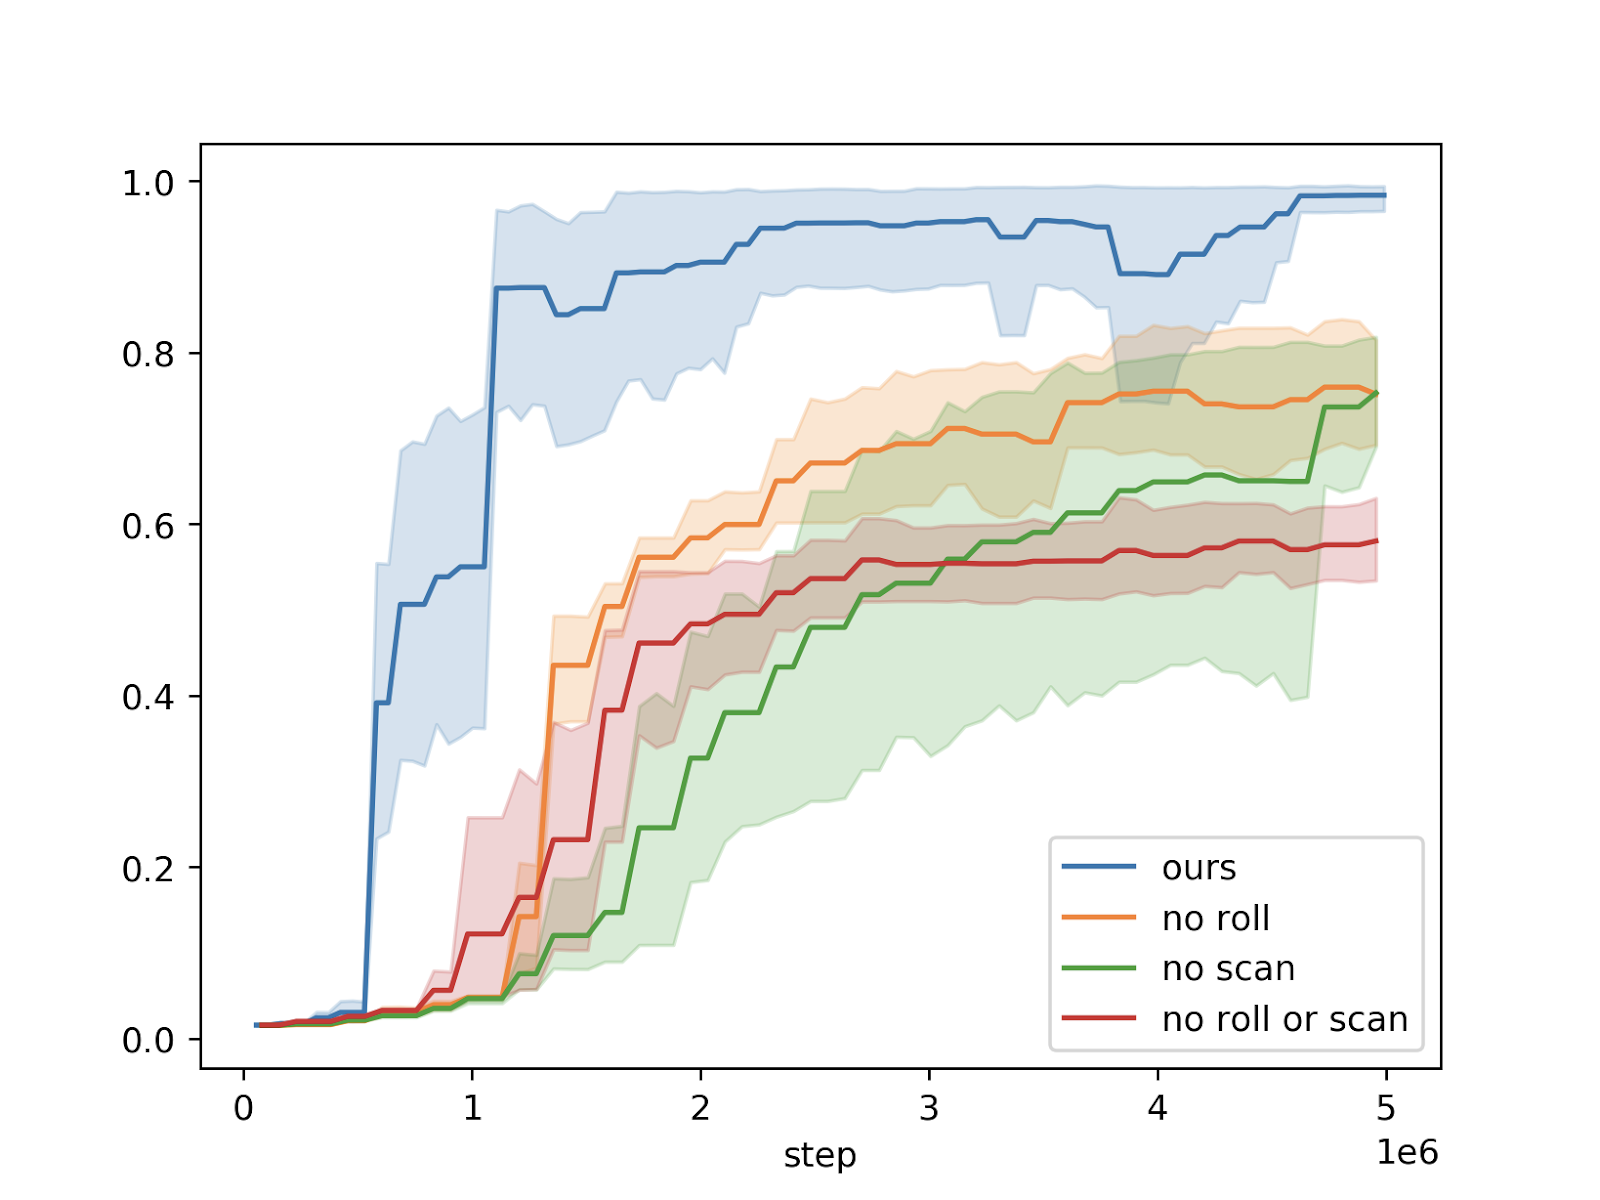
\includegraphics[width=\columnwidth]{figures/eval20}}
    \caption{Evaluation on instructions of length 20}
  \end{subfigure}%
  \begin{subfigure}{.33\textwidth}
    \centering
    \centerline{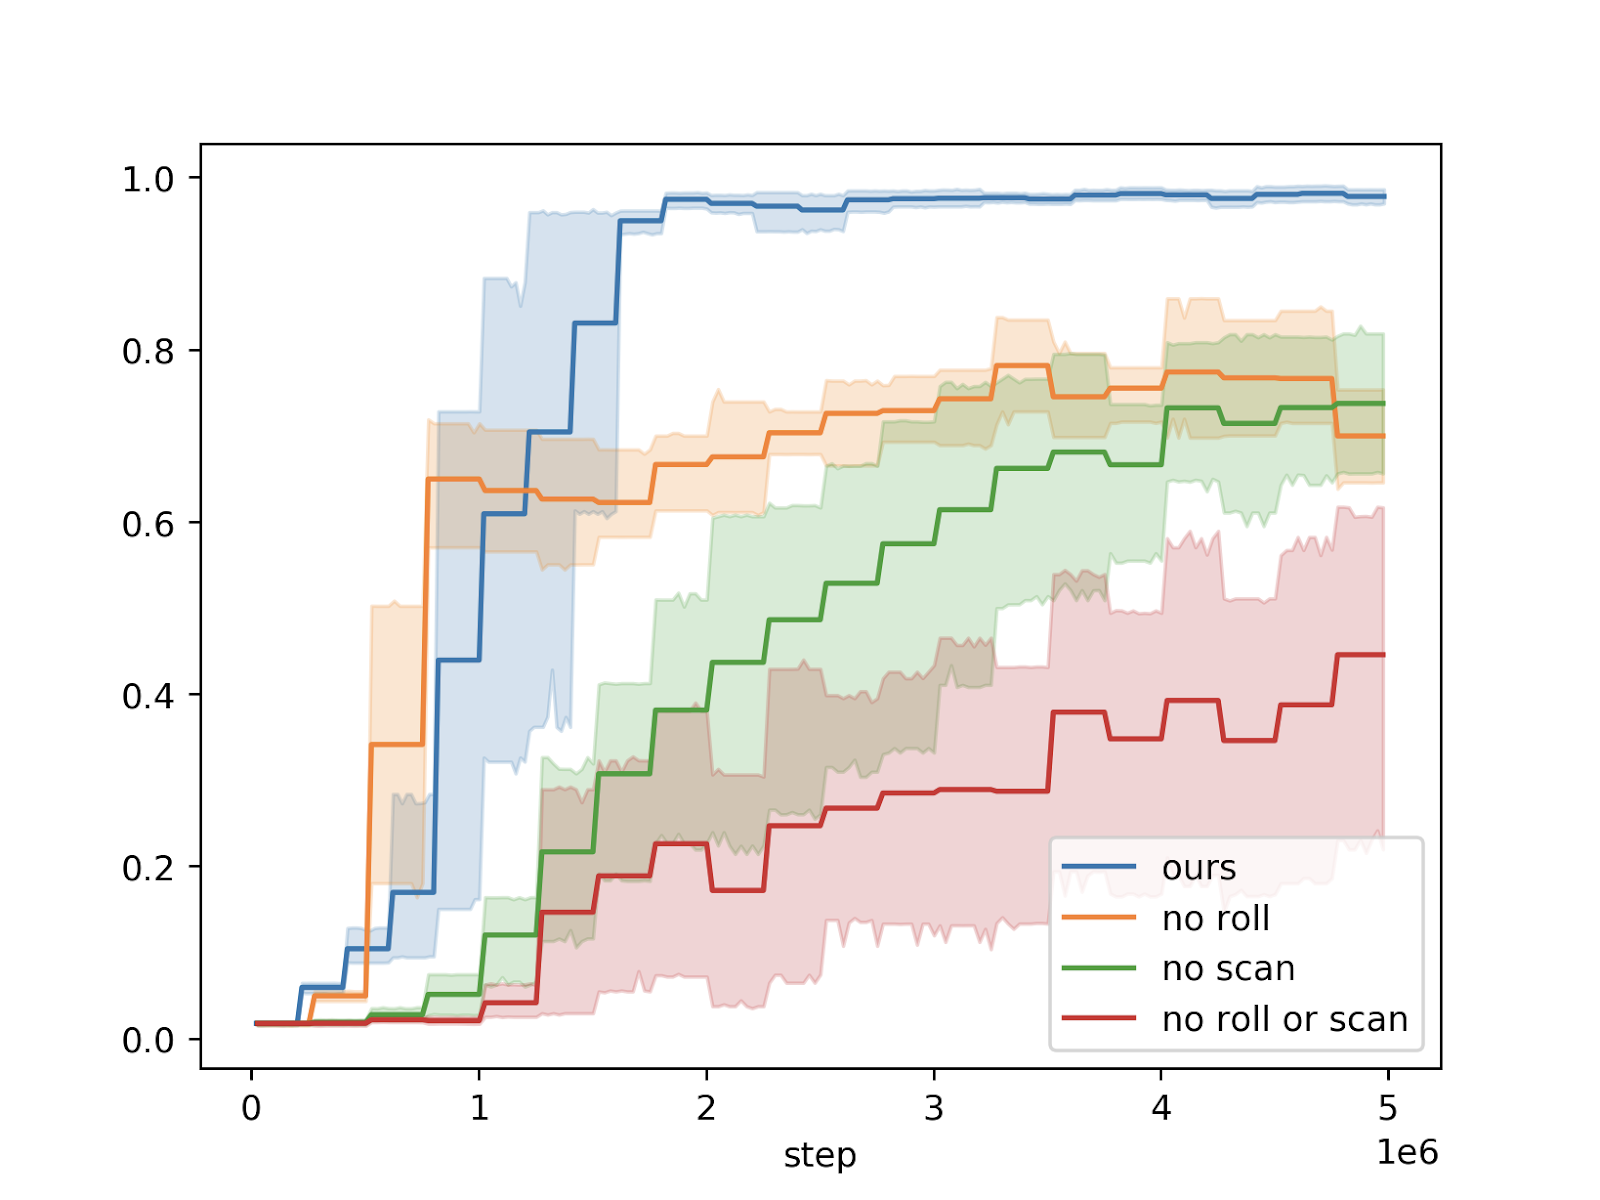
\includegraphics[width=\columnwidth]{figures/eval30}}
    \caption{Evaluation on instructions of length 30}
  \end{subfigure}%
  \begin{subfigure}{.33\textwidth}
    \centering
    \centerline{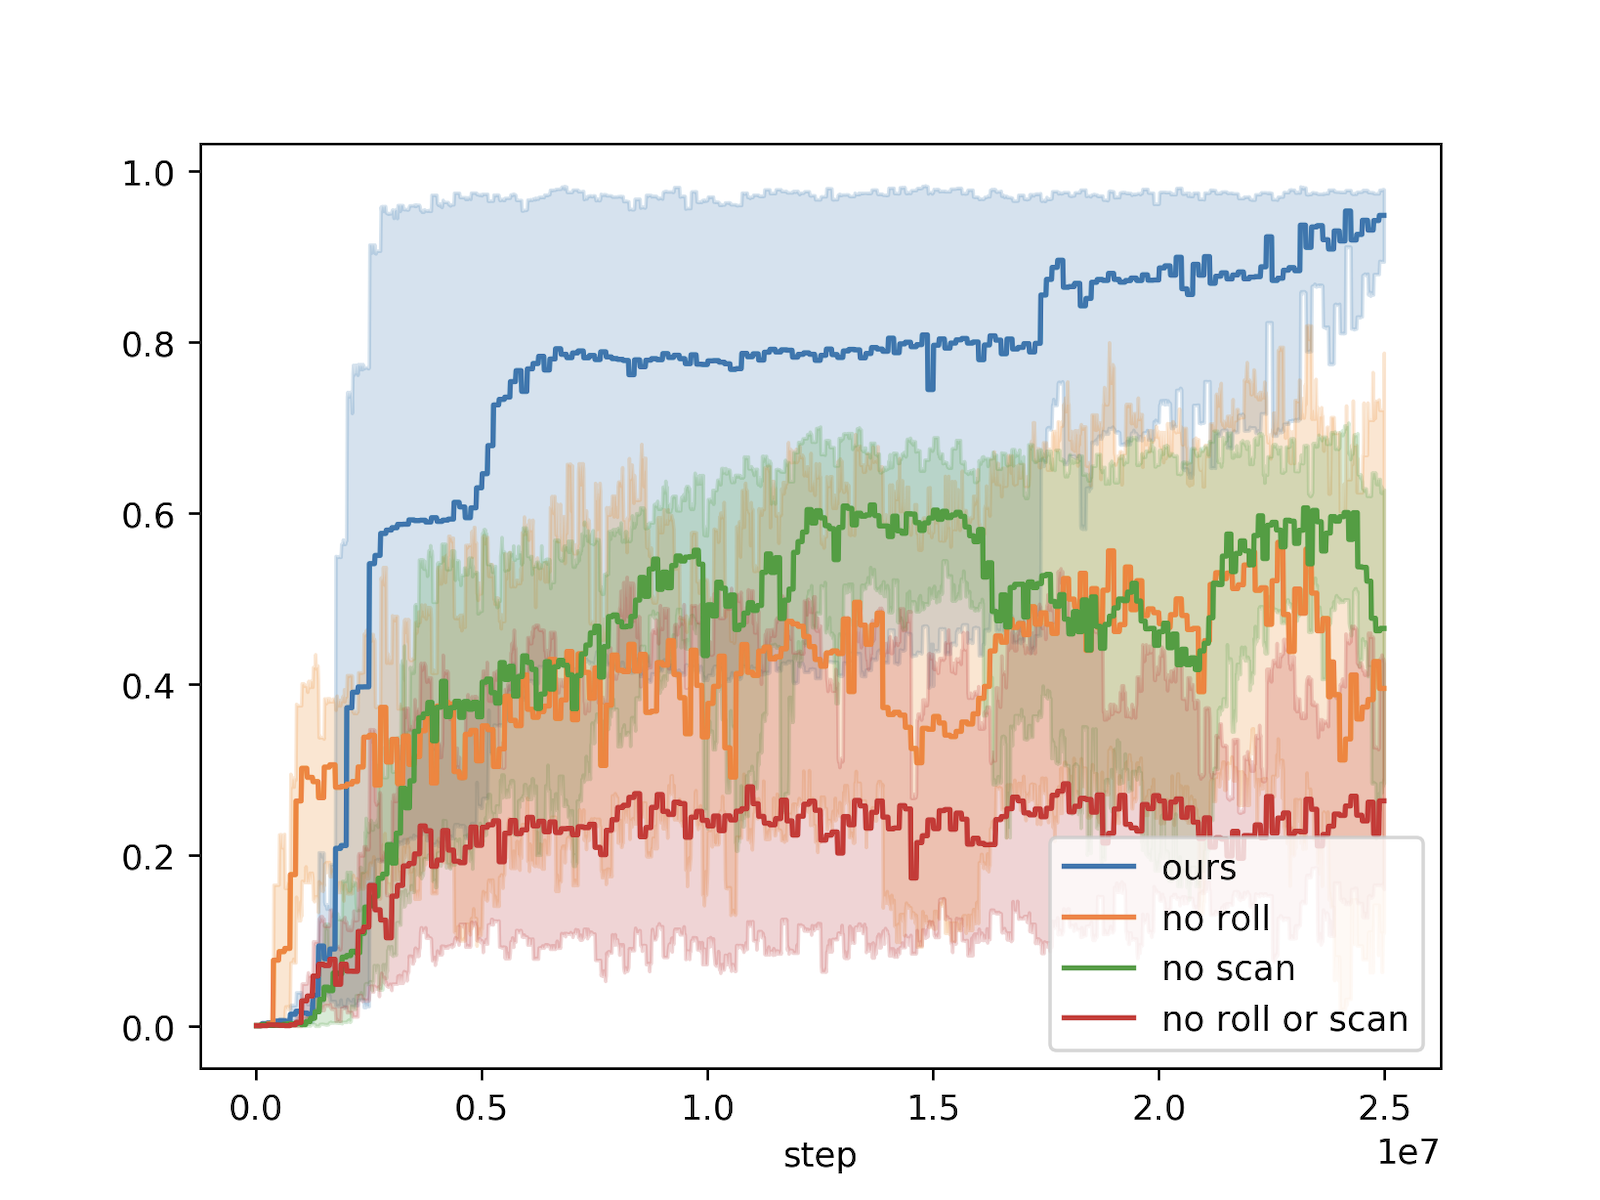
\includegraphics[width=\columnwidth]{figures/eval40}}
    \caption{Evaluation on instructions of length 40}
  \end{subfigure}%
  \caption{This graph compares the performance of our architecture with the
baseline architectures on the minimal environment with subtasks that terminate
in a single time-step.
Details are provided in section \ref{results}.}
  \label{minimal}
\end{figure*}

\subsection{Instruction Scanning}\label{scanning}
Each episode, our architecture generates a graph representation of the
instruction that allows the internal memory to navigate the instruction over the
course of the episode.  From every line in the instruction, we produce
$\ell$ outgoing edges which each correspond to a learned distribution over other lines
in the instruction. To produce each distribution, we feed the embedded representation
of the instruction $\mathbf{M}$ through a bidirectional GRU to produce a
representation $\mathbf{H} \in \mathbb{R}^{2K \times H}$ 
that incorporates global context information. The outputs of the GRU in both
directions are projected to a vector $\mathbf{B} \in (0, 1)^{2K\times \ell
 }$ using a sigmoidal
perceptron. Finally the equation for the distribution over next lines is
\begin{equation}
  \label{P}
  \mathbf{P}_{ij} = \mathbf{B}_{ij}\prod_{k \in (1, -1, 2, -2, \dots)}\left(1 -
  \mathbf{B}_{kj}\right)
\end{equation}
where $\mathbf{P} \in \mathbb{R}^{2K\times\ell }$. Intuitively, for any $1\le j
\le \ell$, 
$\left(\mathbf{P}_{1,j}, \dots, \mathbf{P}_{2K,j}\right)$ is the distribution produced by
sampling a Bernoulli distribution parameterized by $\mathbf{B}_{kj}$ at each index
$k$, concentrically moving away from the first index, and stopping at the first success.
As section \ref{rolling} will explain, $\mathbf{B}_{1j}$ may
correspond to an index other than the first for $\mathbf{I}$ and $\mathbf{M}$.

As in OLSK, movements of the internal memory pointer are a learned
function of the history of selections in memory, of actions and of observations.
Concretely, we generate a hidden state by feeding all of these values each time
step through a Gated Recurrent Network \citet{ChoMGBSB14}:
\begin{equation}
  \label{gru}
  \mathbf{h}_t = \GRU\left(f_\theta\left(\mathbf{x}_t\right),
    \mathbf{M}_{p_{t-1}}, \mathbf{g}_{t-1},
  \mathbf{h}_{t-1}\right)
\end{equation}
where $f_\theta$ is a convolutional neural network. Whereas the
OLSK architecture
projects $\mathbf{h}_{t}$ to the one-step convolution operator described in
section \ref{internal-memory-pointer}, we project $\mathbf{h}_t$ to $\mathbf{u}_t\in \mathbb{R}^\ell$, a weight vector
used to choose among paths previously encoded from the instruction. Thus, the final
distribution over next lines is
$\Cat(\mathbf{P}_{p_t}\tilde{\mathbf{u}}_t)$, where $\tilde{\mathbf{u}}_t =
\softmax\left(\mathbf{u}_t\right)$.


\subsection{Instruction Rolling}
\label{rolling}
This feature takes advantage of the fact that the rules of control flow are
invariant to the position of the current line in the instruction. ``Rolling'' here
refers to a modular operation by which all elements in a tensor are shifted in
one direction such that elements shifted beyond the last position are
re-introduced at the first position. For example, rolling the tensor 
$\begin{bmatrix} 1 & 2 & 3 & 4 & 5 \end{bmatrix}$ by $-2$ generates the tensor
$\begin{bmatrix} 3 & 4 & 5 & 1 & 2 \end{bmatrix}$. 

The relevance to our architecture is that the encoded instruction $\mathbf{M}$ is rolled to the current memory index
$p_t$ before feeding it to the bidirectional GRU. In other words, the forward GRU takes lines in the
order $(p_t, p_t + 1, \dots, K, 1, \dots, p_t - 1)$, running from the current
line, wrapping around the last line of the instruction, and returning to the line
before the current line. Thus, the operations described in section \ref{scanning} are all performed
relative to the current active line in memory. That is, $\mathbf{B}_{i\cdot}$ in
equation \ref{P} refers to the row of $\mathbf{B}$ corresponding to the $(p_t +
i)^{\text{th}}$ index of $\mathbf{M}$.

\subsection{Algorithm Description}
In summary, each time-step our algorithm 
\begin{enumerate}
  \item rolls the embedded instruction $\mathbf{M}$ so that the index
    corresponding to the pointer $p_t$ is first.
  \item passes the embedded instruction through a bidirectional GRU in order to
    incorporate global context information.
  \item uses the \texttt{scan} function to produce $\ell$ distributions with
    dimension $2K$ (see Algorithm \ref{scan} for pseudocode).
  \item passes the current observation and the $p_t^{\text{th}}$ index of
    $\mathbf{M}$ through a GRU controller in order to generate hidden state
    $\mathbf{h}_t$.
  \item projects $\mathbf{h}_t$ to the  $\ell$-dimensional probability vector
    $\mathbf{u}$ and to the distribution from which the next subtask parameter
    $\mathbf{g}_t$ is sampled.
  \item uses $\tilde{\mathbf{u}} = \softmax(\mathbf{u})$ to produce a weighted
    sum of the $\ell$ distributions in matrix $\mathbf{P}$. Intuitively,
    $\tilde{\mathbf{u}}$ chooses among the outgoing edges from the current node.
  \item uses the resulting distribution to sample $d_t$ which is used to produce
    $p_{t+1} = p_t + d_t$.
\end{enumerate}
Pseudocode is provided in Algorithm ~\ref{algo}.

\section{Experiments}
\label{experiments}
In order to validate the effectiveness of our algorithm, we ran two sets of
experiments in different environments. The first environment is minimal,
intended only to test
the agent's capability to move the internal memory pointer through an instruction
involving complex control flow. The second involves temporally-extended subtasks
of the kind discussed earlier and non-trivial logical conditions. For all
experiments the maximum possible reward is 1.

\begin{figure*}[th]
  \centering
  \begin{subfigure}{.5\textwidth}
    \centering
    \centerline{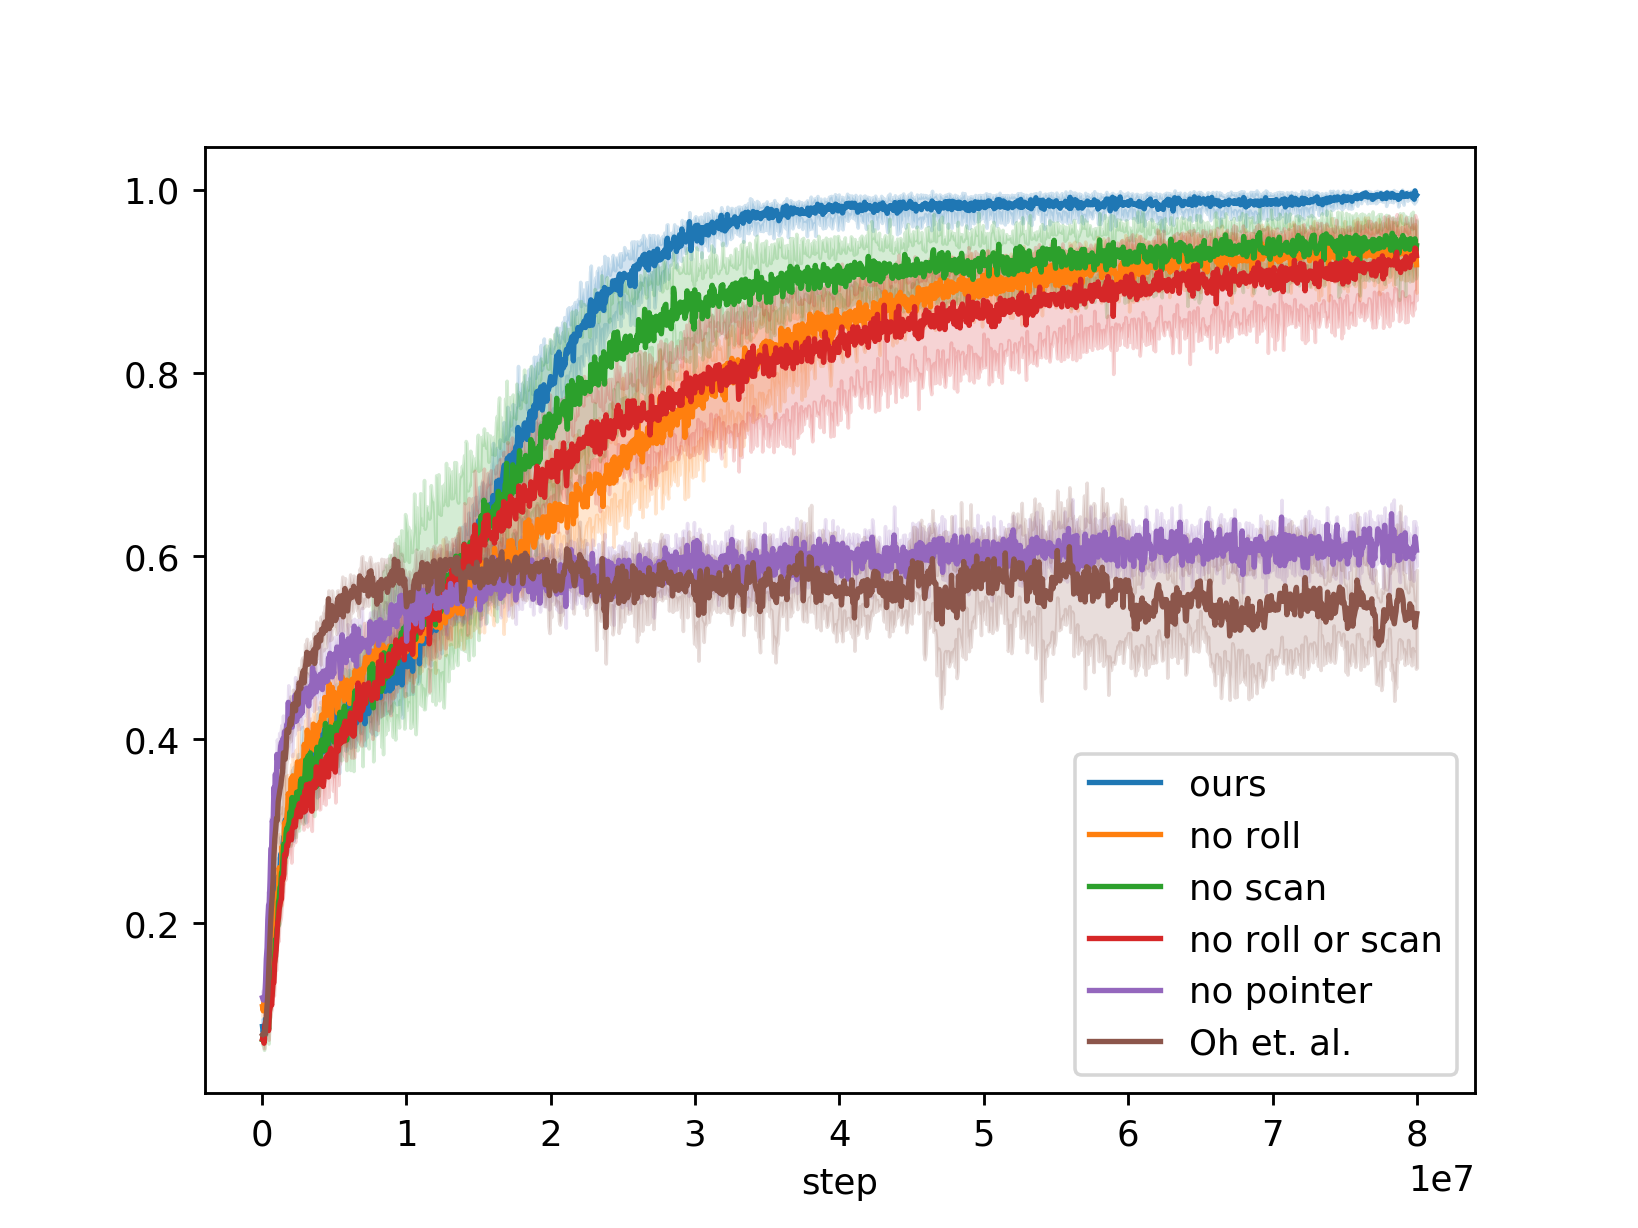
\includegraphics[
    width=\columnwidth]{figures/complex-train}}
    \caption{Training reward on instructions with lengths sampled uniformly
    between 1 and 10}
  \end{subfigure}%
  \begin{subfigure}{.5\textwidth}
    \centering
    \centerline{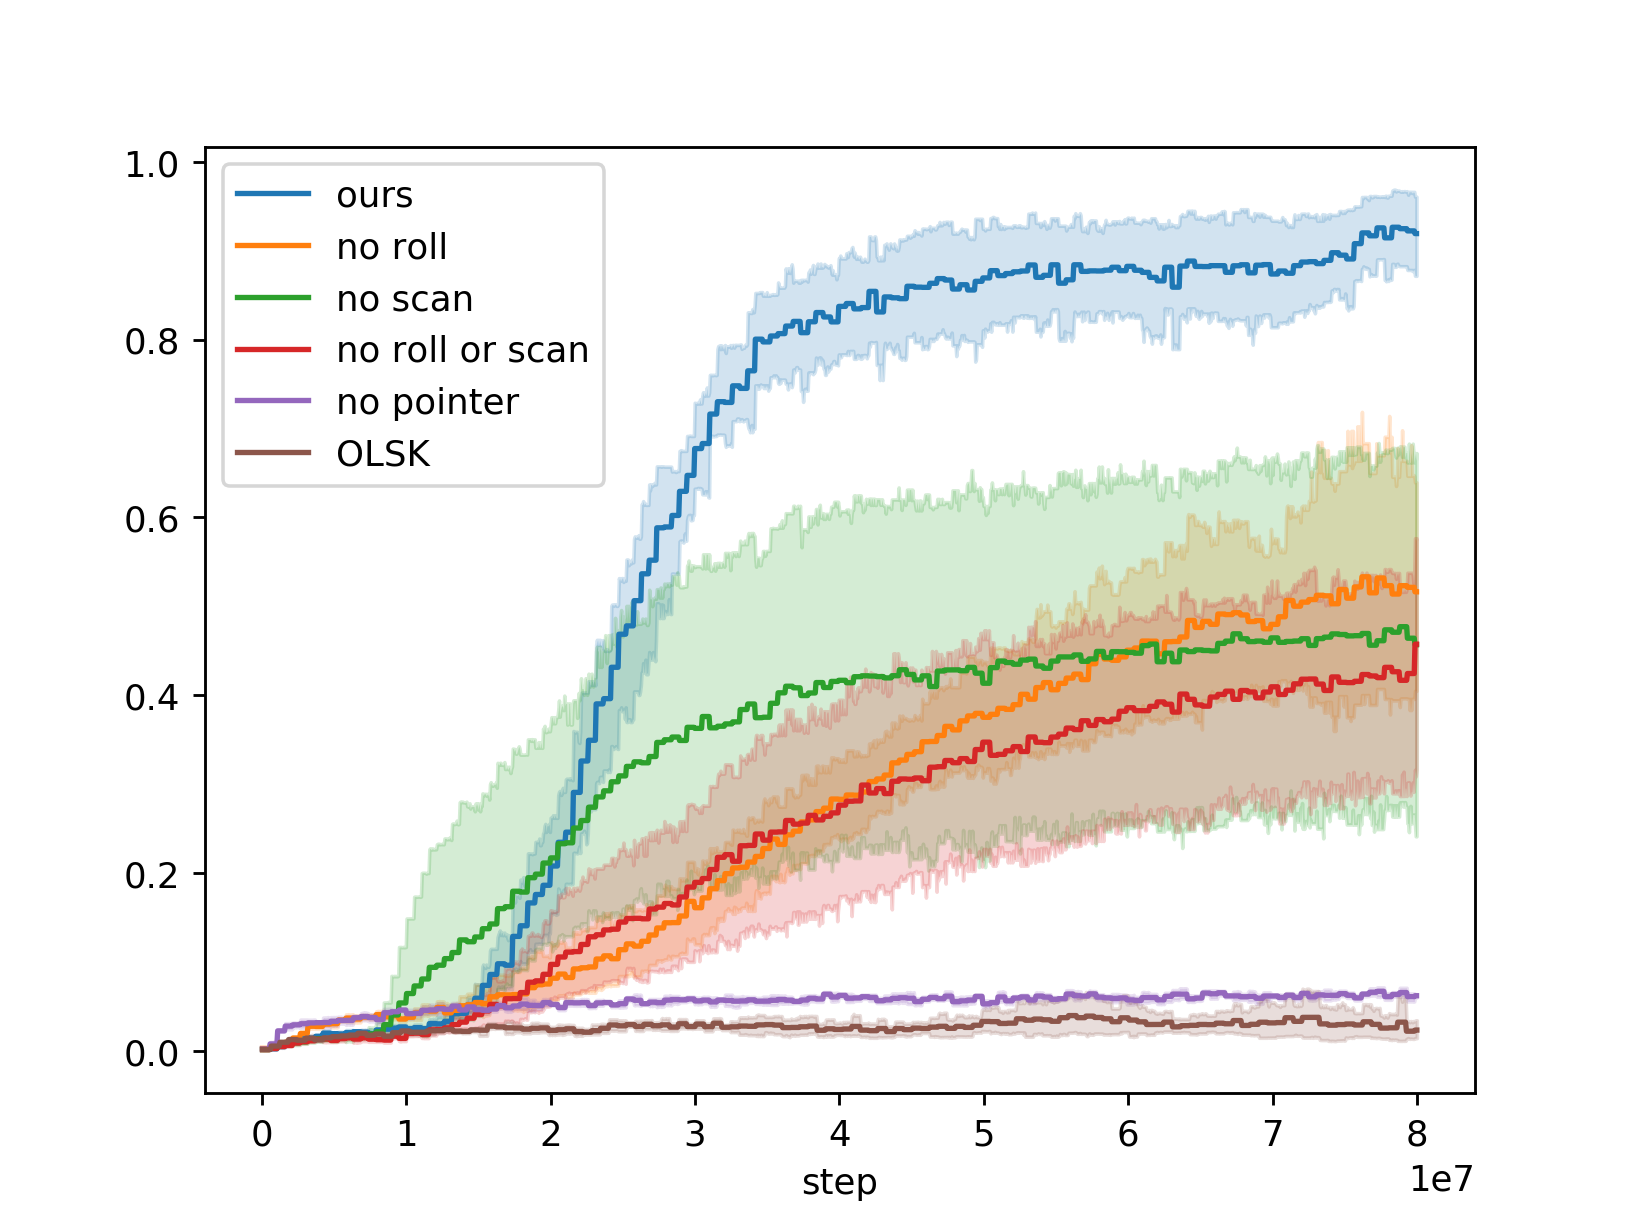
\includegraphics[
    width=\columnwidth]{figures/complex-eval}}
    \caption{Evaluation reward on instructions of length 20}
  \end{subfigure}%
  \caption{These graphs depict performance on the complex $6\times6$ environment
    with temporally extended subtasks. Details are provided in
section \ref{results}.}
  \label{complex}
\end{figure*}

\begin{figure}[t]
\vskip 0.2in
\centerline{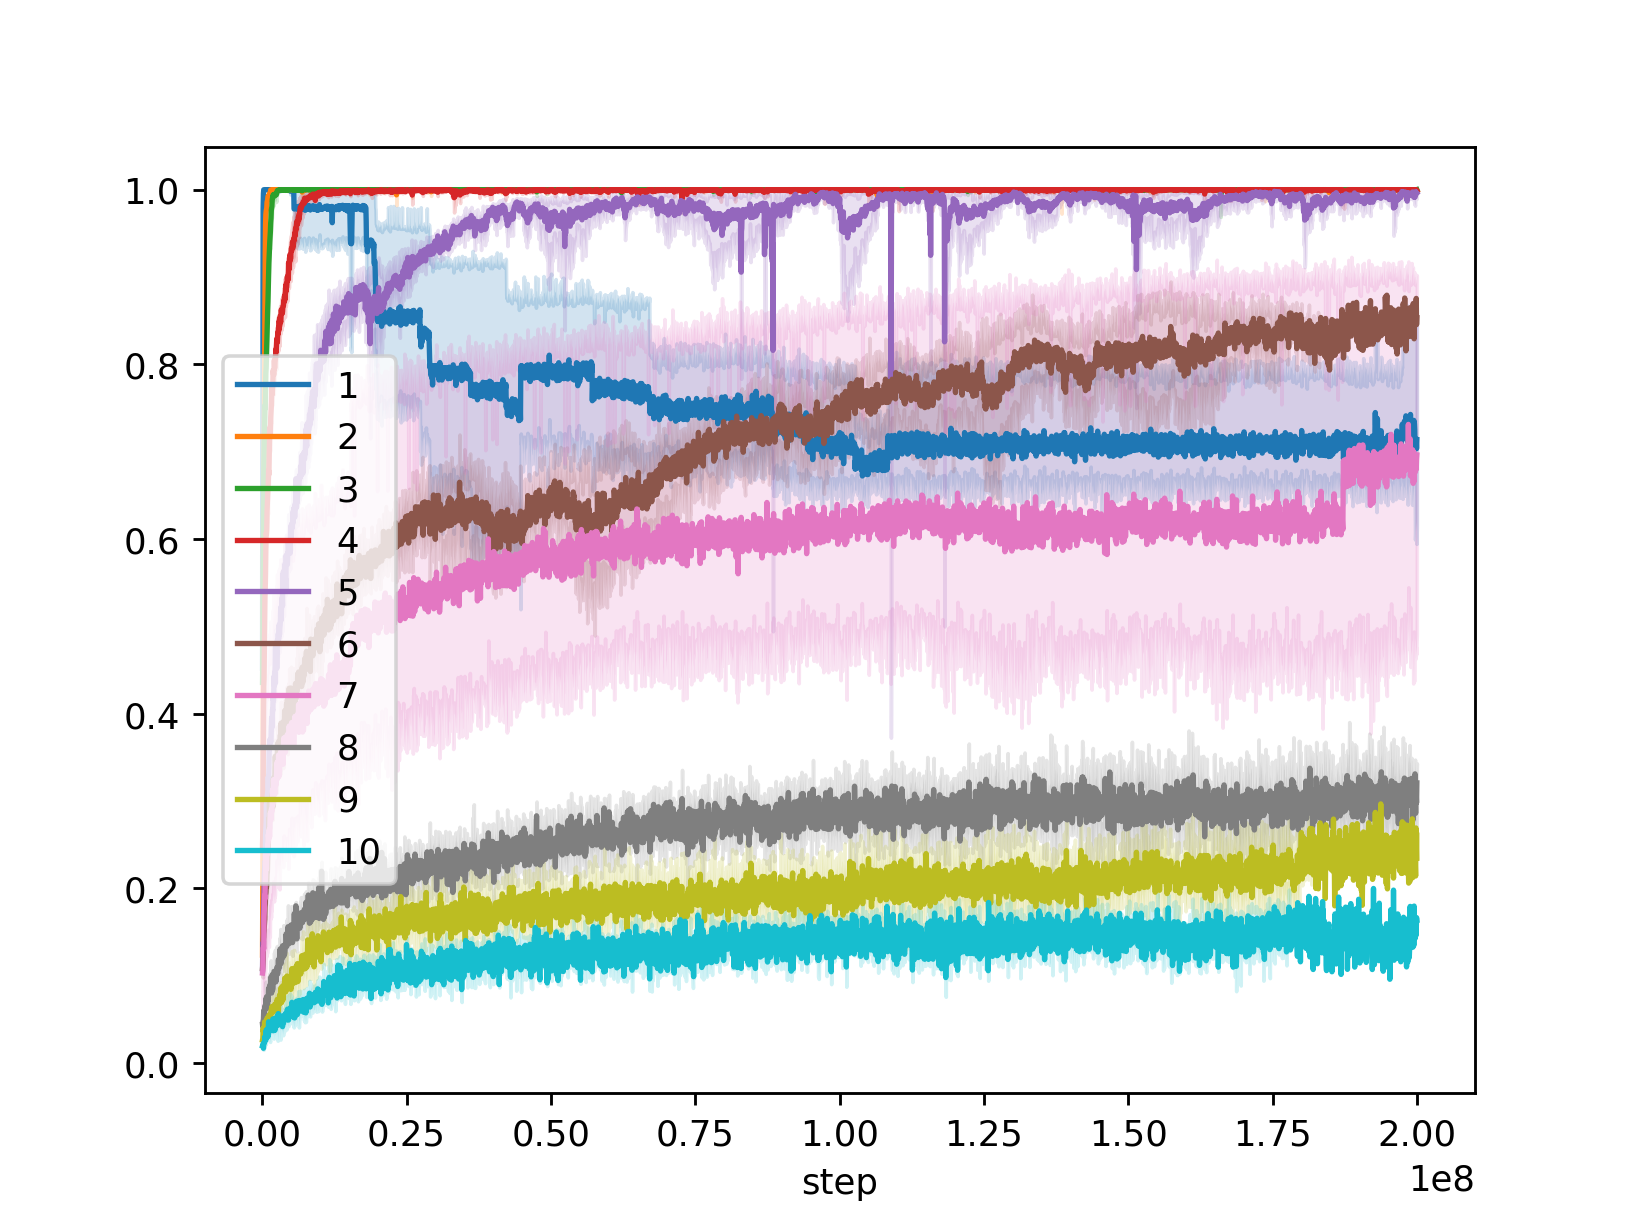
\includegraphics[width=\columnwidth]{simple-rewards.png}}
\caption{Training performance of the ``simple architecture'' on the minimal
environment. Each line corresponds to the number of lines per instruction.
Note that all agents trained on tasks with lengths greater than 5 fail to
converge to the maximum possible reward of 1.}
\label{simple-rewards}
\vskip -0.2in
\end{figure}

\subsection{Implementation details}
All agents were trained using the Proximal Policy Optimization algorithm
\cite{schulman2017proximal}. Details are provided in Appendix \ref{training}.
Each agent generates behavior using 150 parallel processes. Each time-step the
observation is fed through a single-layer convolutional network with kernel-size
1 followed by max-pooling layer. We use a single layer perceptron with a
Rectified Linear Unit \cite{nair2010rectified} to project the GRU output
$\mathbf{h}_t$ to both $\mathbf{u}$ and the distribution over
subtask parameters (see equation \ref{gru}).

For the complex environment, a few modifications were made to the base algorithm
inspired by OLSK. Because of the temporally-extended nature of subtasks, we
found it beneficial to incorporate gates into the algorithm that prevent changes
to certain internal parameters, especially when a subtask is not yet complete.
Specifically, OLSK use a gate to regulate changes to the internal memory
pointer, the hidden state, and the subtask parameter.
We make two changes to the architecture described in OLSK:
\begin{enumerate}
  \item OLSK use ``soft-gates'', producing a scalar value $c_t \in (0, 1)$ that
    interpolates old values with new values. Thus when $c_t \approx 0$, the old
    value is retained and when $c_t \approx 1$, the new value is adopted. Toward
    the end of training, 
    OLSK recommend switching to hard-updates, sampling values from a learned
    distribution which is trained with reinforcement learning. However we find
    that it is beneficial to use hard-updates from the beginning of training.
  \item Instead of using a single gate, we use a separate gate for the
    subtask parameter and for the internal memory pointer.
Concretely, we project $\mathbf{h}_t$ to two Bernoulli distributions, fom which
we sample the gate values, $c_g$ and $c_p$. Having produced tentative new values
for the subtask parameter $\tilde{\mathbf{g}}_t$ and the internal pointer
$\tilde{p}_t$, we set $\mathbf{g}_t = c_g\tilde{\mathbf{g}}_t + (1 -
c_g)\mathbf{g}_{t-1}$ and  $p_t = c_p\tilde{p}_t + (1 - c_p)p_{t-1}$.

  \item Like OLSK, we divide the recurrent hidden state $\mathbf{h}_t$ into two
    parts, one updated every time-step and one updated only when the value of
    the gates is one. However, we condition the distribution from which the gate
    values are sampled exclusively on the hidden state that is updated each
    time-step and we condition $V_t$ (the value estimate), $\mathbf{u}_t$ and
    the subtask parameter distribution on the hidden state that is only updated
    when the gate values are 1.
\end{enumerate}

Pseudocode for the full algorithm used on the complex environment is provided in
Appendix \ref{full-algorithm}.

\subsection{Baselines}
In our experiments, we ablate the main features of our algorithm in order to
test their effectiveness. We present five baselines:
\begin{itemize}
  \item \textbf{No scan:} This baseline removes the instruction scanning feature by
    taking the last output of $\BIGRU(\mathbf{M}^{p_t})$ and projecting it to
    a distribution over possible forward and backward pointer movements.
    Movements that go beyond the beginning or end of the instruction are clipped.
  \item \textbf{No roll:} This baseline does not roll $\mathbf{M}$ before feeding
    it to the bidirectional GRU as described in section \ref{rolling}.
  \item \textbf{No roll or scan:} This baseline combines both ablations.
  \item \textbf{No pointer:} This baseline removes the internal memory pointer.
    Instead, it feeds a representation $\mathbf{H}'$ of the instruction
    $\mathbf{I}$ along with the observation $\mathbf{x}_t$ to a GRU controller
    which directly outputs a distribution over actions $\pi_\theta(\cdot)$ and a
    value $V_t$. We generate $\mathbf{H}'$ by feeding the embedded instruction
    $\mathbf{M}$ through a bidirectional GRU and concatenating the last outputs
    in both directions. See figure \ref{no-pointer}. 
  \item \textbf{OLSK} This baseline reproduces the algorithm described in
    OLSK.
  \item \textbf{Simple:} The ``simple'' architecture for which figure
    \ref{simple-rewards} depicts performance on training tasks. This
    architecture is almost identical to the \textbf{No Pointer} baseline except
    that the embedded instruction $\mathbf{M}$ is fed directly to the GRU
    controller. Note that this prevents the architecture from generalizing to
    longer instructions because the controller requires fixed-length inputs. We
    therefore present only training results for this architecture.
\end{itemize}
Pseudocode for all the baselines is also included in Appendix \ref{baselines}.

\subsection{Minimal Environment}
In the minimal setting, subtasks are not
temporally extended -- as soon as the agent outputs the correct subtask
parameter, the subtask is complete and the external program counter advances.
Moreover, conditions are evaluated according to a simple ``condition bit'' which
is randomly 1 or 0, with 50\% probability. If the condition bit is 1,
\texttt{if}-conditions and \texttt{while}-conditions pass; otherwise they fail.

\subsection{Complex Environment}
In this setting, the agent dictates subtask parameters to a pretrained
lower-level agent who executes them. The environment is a $6\times 6$ grid world
with randomly spawned objects. The lower-level agent must navigate to the object
and perform the interaction (visit, pickup, or transform) corresponding to the
subtask parameter chosen by the higher-level agent. Thus, subtasks may take several time-steps to
complete. Moreover, conditions are parameterized by \textit{objects} and they
are evaluated according to whether the object exists. For example, the statement
\texttt{If cat} evaluates to true, if there is a cat somewhere in the
environment, and to false otherwise.


 
\subsection{Results}
\label{results}
Figures \ref{minimal} and \ref{complex} compare the performance of our
architecture with several baselines. 
Unless otherwise specified, each graph plots the rewards that these architectures achieved on \textit{longer
length} instructions.
 Note that all graphs depict the performance of agents trained on instructions with lengths drawn uniformly between 1 and 10. Thus
the graphs corresponding to longer instructions measure the generalization
capability of each architecture. Each line is the average reward achieved by the
150 parallel behavior processes over the course of
200 steps of evaluation. The error bars represent five separate distinct random
seeds ($150 \times 5$ total processes).

\subsection{Analysis}
Identifying failure modes can be difficult with both our algorithm and the
baselines because identifiable failures may be far downstream of the root cause.
For example, we observe that on the longer evaluation instructions, the
\textbf{No roll} baseline consistently mis-evaluates conditions, especially in
while loops. However, the architecture responsible for evaluating conditions is
identical between the \textbf{No roll} baseline and our architecture. We infer that this
part of the architecture was somehow poorly trained due to failures in other parts
of the architecture that do differ somehow from our architecture.

With this caveat, a few broad conclusions can be drawn from the experimental
results. As one would expect, evaluation performance lags behind training
performance since errors are compounded on the longer instructions -- an
instruction that is twice as long offers twice as many opportunities to make a
mistake. Consequently, strong performance on the evaluation tasks requires
nearly flawless performance on the training instruction. Any architecture that fails to
converge on the training tasks will have demonstrate dismal performance on the
evaluation tasks.  We observe that all architectures with both an internal memory pointer and the
capacity to move from any memory index to any other memory index are able to
achieve near optimal performance on their training tasks. 

\subsubsection{Our architecture}
Reviewing the behavior of a fully trained agent, we did not observe any
prominent error trends unique to our architecture. That is, certain failure
modes emerged among all the architectures but were less prominent in ours,
accounting for the improved performance. Common points of failure include
terminating a while loop early or late, executing the previous action instead of
the current, or missing a long jump (that is, the architecture sometimes fails
to navigate to the next active line if it comes long after the current line due
to failed condition blocks).

We attribute some of these failures to artifacts that can develop in recurrent
architectures -- spurious correlations with past observations may form, leading
to local optima that may take a long time to escape.

\subsubsection{No roll}
Without rolling, the pointer movements that get encoded in $\mathbf{P}_t$ become
generic, no longer a function of the input instruction. The reason is that there
is not way for the bidirectional GRU to know the current index of the memory pointer 
and what jumps might be appropriate from there (whereas with the roll operation,
the current index of the memory pointer is always the first input to the
bidirectional GRU). Thus, the agent learns a series of standard movements common
in the randomly generated instructions -- move forward one line (the most common
movement), move backward two lines (the mean length of a while loop is two
lines), etc.

As one might expect, these generic movements only work for a subset of
instructions. One common error that this baseline exhibits is jumping to the
wrong location, especially for uncommon movements. We also note that this
baseline often mis-evaluates condition statements and we hypothesize that this
is a ``downstream'' error of the kind we discussed earlier.

\subsubsection{No scan / No roll or scan}
We observe that agents that do not use the scan function tend to learn a
strategy that involves walking the memory pointer linearly through the
instruction, outputting no-op actions inside failing condition blocks. While in
principle this is a valid strategy for executing instructions of the kind
described in this document, we observe a common tendency on the part of these agents to 
advance the memory pointer prematurely (before performing the appropriate
subtask) or to mis-evaluate while loops. We hypothesize that oveloading the
GRU controller complicates the learning process, dissipating the effects of the
learning signal, and exposing the learning process to a variety of local optima.

\subsubsection{No pointer baseline}
On expectation, this baseline succeeds on its first subtask and fails
thereafter. Instead of consistently outputing a single subtask parameter until
the associated subtask is complete, the agent chooses a different subtask
parameter nearly every time-step, mostly choosing among those that correspond to
sutbasks appearing early in the instruction.

Any architecture that succeeds on the kinds of tasks that we describe in this
work must learn a very complex representation of the instruction that encodes
all possible pathways through it. We hypothesize that the search space for
representations is sufficiently large and the number of local optima in this
space sufficiently numerous that an unstructured recurrent network like a GRU
either has little chance of discovering that representation or a more extensive
hyperparameter search is necessary than that undertaken in this work.

\subsubsection{OLSK baseline}
This baseline learns a strategy of sweeping the attention weights across
the entire instruction and essentially delegating the choice of action entirely
to the GRU controller. This strategy encounters many of the same difficulties
and the \textbf{No pointer} baseline, failing to properly encode the possible
paths through the instruction and roughly approximating them with high error.

\section{Conclusion}
This work studies a special but important subset of multi-task reinforcement
learning problems, namely instructions with complex control-flow. We consider
problems of this nature an important stepping stone toward natural language
instructions and toward agents capable of arbitrarily complex logic. We hope
that future work will explore instructions that involve greater complexity,
including conditionals with more complex predicates, higher-dimensional
observations, and noisy natural-language inputs.

%\section{To do}
%\begin{itemize}
  %\item Add more related works
  %\item Add diagram of edge length performance.
  %\item If time permits, add other baselines to single-step environment.
%\end{itemize}

%\section{Electronic Submission}
%\label{submission}

%Submission to ICML 2019 will be entirely electronic, via a web site
%(not email). Information about the submission process and \LaTeX\ templates
%are available on the conference web site at:
%\begin{center}
%\textbf{\texttt{http://icml.cc/}}
%\end{center}

%The guidelines below will be enforced for initial submissions and
%camera-ready copies. Here is a brief summary:
%\begin{itemize}
%\item Submissions must be in PDF\@.
%\item The maximum paper length is \textbf{8 pages excluding references and
    %acknowledgements, and 12 pages including references and acknowledgements}
    %(pages 9 through 12 must contain only references and acknowledgements).
%\item \textbf{Do not include author information or acknowledgements} in your
    %initial submission.
%\item Your paper should be in \textbf{10 point Times font}.
%\item Make sure your PDF file only uses Type-1 fonts.
%\item Place figure captions \emph{under} the figure (and omit titles from inside
    %the graphic file itself). Place table captions \emph{over} the table.
%\item References must include page numbers whenever possible and be as complete
    %as possible. Place multiple citations in chronological order.
%\item Do not alter the style template; in particular, do not compress the paper
    %format by reducing the vertical spaces.
%\item Keep your abstract brief and self-contained, one paragraph and roughly
    %4--6 sentences. Gross violations will require correction at the
    %camera-ready phase. The title should have content words capitalized.
%\end{itemize}

%\subsection{Submitting Papers}

%\textbf{Paper Deadline:} The deadline for paper submission that is
%advertised on the conference website is strict. If your full,
%anonymized, submission does not reach us on time, it will not be
%considered for publication. There is no separate abstract submission.

%\textbf{Anonymous Submission:} ICML uses double-blind review: no identifying
%author information may appear on the title page or in the paper
%itself. Section~\ref{author info} gives further details.

%\textbf{Simultaneous Submission:} ICML will not accept any paper which,
%at the time of submission, is under review for another conference or
%has already been published. This policy also applies to papers that
%overlap substantially in technical content with conference papers
%under review or previously published. ICML submissions must not be
%submitted to other conferences during ICML's review period. Authors
%may submit to ICML substantially different versions of journal papers
%that are currently under review by the journal, but not yet accepted
%at the time of submission. Informal publications, such as technical
%reports or papers in workshop proceedings which do not appear in
%print, do not fall under these restrictions.

%\medskip

%Authors must provide their manuscripts in \textbf{PDF} format.
%Furthermore, please make sure that files contain only embedded Type-1 fonts
%(e.g.,~using the program \texttt{pdffonts} in linux or using
%File/DocumentProperties/Fonts in Acrobat). Other fonts (like Type-3)
%might come from graphics files imported into the document.

%Authors using \textbf{Word} must convert their document to PDF\@. Most
%of the latest versions of Word have the facility to do this
%automatically. Submissions will not be accepted in Word format or any
%format other than PDF\@. Really. We're not joking. Don't send Word.

%Those who use \textbf{\LaTeX} should avoid including Type-3 fonts.
%Those using \texttt{latex} and \texttt{dvips} may need the following
%two commands:

%{\footnotesize
%\begin{verbatim}
%dvips -Ppdf -tletter -G0 -o paper.ps paper.dvi
%ps2pdf paper.ps
%\end{verbatim}}
%It is a zero following the ``-G'', which tells dvips to use
%the config.pdf file. Newer \TeX\ distributions don't always need this
%option.

%Using \texttt{pdflatex} rather than \texttt{latex}, often gives better
%results. This program avoids the Type-3 font problem, and supports more
%advanced features in the \texttt{microtype} package.

%\textbf{Graphics files} should be a reasonable size, and included from
%an appropriate format. Use vector formats (.eps/.pdf) for plots,
%lossless bitmap formats (.png) for raster graphics with sharp lines, and
%jpeg for photo-like images.

%The style file uses the \texttt{hyperref} package to make clickable
%links in documents. If this causes problems for you, add
%\texttt{nohyperref} as one of the options to the \texttt{icml2019}
%usepackage statement.


%\subsection{Submitting Final Camera-Ready Copy}

%The final versions of papers accepted for publication should follow the
%same format and naming convention as initial submissions, except that
%author information (names and affiliations) should be given. See
%Section~\ref{final author} for formatting instructions.

%The footnote, ``Preliminary work. Under review by the International
%Conference on Machine Learning (ICML). Do not distribute.'' must be
%modified to ``\textit{Proceedings of the
%$\mathit{36}^{th}$ International Conference on Machine Learning},
%Long Beach, USA, 2019.
%Copyright 2019 by the author(s).''

%For those using the \textbf{\LaTeX} style file, this change (and others) is
%handled automatically by simply changing
%$\mathtt{\backslash usepackage\{icml2019\}}$ to
%$$\mathtt{\backslash usepackage[accepted]\{icml2019\}}$$
%Authors using \textbf{Word} must edit the
%footnote on the first page of the document themselves.

%Camera-ready copies should have the title of the paper as running head
%on each page except the first one. The running title consists of a
%single line centered above a horizontal rule which is $1$~point thick.
%The running head should be centered, bold and in $9$~point type. The
%rule should be $10$~points above the main text. For those using the
%\textbf{\LaTeX} style file, the original title is automatically set as running
%head using the \texttt{fancyhdr} package which is included in the ICML
%2019 style file package. In case that the original title exceeds the
%size restrictions, a shorter form can be supplied by using

%\verb|\icmltitlerunning{...}|

%just before $\mathtt{\backslash begin\{document\}}$.
%Authors using \textbf{Word} must edit the header of the document themselves.

%\section{Format of the Paper}

%All submissions must follow the specified format.

%\subsection{Length and Dimensions}

%Papers must not exceed eight (8) pages, including all figures, tables,
%and appendices, but excluding references and acknowledgements. When references and acknowledgements are included,
%the paper must not exceed ten (10) pages.
%Acknowledgements should be limited to grants and people who contributed to the paper.
%Any submission that exceeds
%this page limit, or that diverges significantly from the specified format,
%will be rejected without review.

%The text of the paper should be formatted in two columns, with an
%overall width of 6.75~inches, height of 9.0~inches, and 0.25~inches
%between the columns. The left margin should be 0.75~inches and the top
%margin 1.0~inch (2.54~cm). The right and bottom margins will depend on
%whether you print on US letter or A4 paper, but all final versions
%must be produced for US letter size.

%The paper body should be set in 10~point type with a vertical spacing
%of 11~points. Please use Times typeface throughout the text.

%\subsection{Title}

%The paper title should be set in 14~point bold type and centered
%between two horizontal rules that are 1~point thick, with 1.0~inch
%between the top rule and the top edge of the page. Capitalize the
%first letter of content words and put the rest of the title in lower
%case.

%\subsection{Author Information for Submission}
%\label{author info}

%ICML uses double-blind review, so author information must not appear. If
%you are using \LaTeX\/ and the \texttt{icml2019.sty} file, use
%\verb+\icmlauthor{...}+ to specify authors and \verb+\icmlaffiliation{...}+ to specify affiliations. (Read the TeX code used to produce this document for an example usage.) The author information
%will not be printed unless \texttt{accepted} is passed as an argument to the
%style file.
%Submissions that include the author information will not
%be reviewed.

%\subsubsection{Self-Citations}

%If you are citing published papers for which you are an author, refer
%to yourself in the third person. In particular, do not use phrases
%that reveal your identity (e.g., ``in previous work \cite{langley00}, we
%have shown \ldots'').

%Do not anonymize citations in the reference section. The only exception are manuscripts that are
%not yet published (e.g., under submission). If you choose to refer to
%such unpublished manuscripts \cite{anonymous}, anonymized copies have
%to be submitted
%as Supplementary Material via CMT\@. However, keep in mind that an ICML
%paper should be self contained and should contain sufficient detail
%for the reviewers to evaluate the work. In particular, reviewers are
%not required to look at the Supplementary Material when writing their
%review.

%\subsubsection{Camera-Ready Author Information}
%\label{final author}

%If a paper is accepted, a final camera-ready copy must be prepared.
%%
%For camera-ready papers, author information should start 0.3~inches below the
%bottom rule surrounding the title. The authors' names should appear in 10~point
%bold type, in a row, separated by white space, and centered. Author names should
%not be broken across lines. Unbolded superscripted numbers, starting 1, should
%be used to refer to affiliations.

%Affiliations should be numbered in the order of appearance. A single footnote
%block of text should be used to list all the affiliations. (Academic
%affiliations should list Department, University, City, State/Region, Country.
%Similarly for industrial affiliations.)

%Each distinct affiliations should be listed once. If an author has multiple
%affiliations, multiple superscripts should be placed after the name, separated
%by thin spaces. If the authors would like to highlight equal contribution by
%multiple first authors, those authors should have an asterisk placed after their
%name in superscript, and the term ``\textsuperscript{*}Equal contribution"
%should be placed in the footnote block ahead of the list of affiliations. A
%list of corresponding authors and their emails (in the format Full Name
%\textless{}email@domain.com\textgreater{}) can follow the list of affiliations.
%Ideally only one or two names should be listed.

%A sample file with author names is included in the ICML2019 style file
%package. Turn on the \texttt{[accepted]} option to the stylefile to
%see the names rendered. All of the guidelines above are implemented
%by the \LaTeX\ style file.

%\subsection{Abstract}

%The paper abstract should begin in the left column, 0.4~inches below the final
%address. The heading `Abstract' should be centered, bold, and in 11~point type.
%The abstract body should use 10~point type, with a vertical spacing of
%11~points, and should be indented 0.25~inches more than normal on left-hand and
%right-hand margins. Insert 0.4~inches of blank space after the body. Keep your
%abstract brief and self-contained, limiting it to one paragraph and roughly 4--6
%sentences. Gross violations will require correction at the camera-ready phase.

%\subsection{Partitioning the Text}

%You should organize your paper into sections and paragraphs to help
%readers place a structure on the material and understand its
%contributions.

%\subsubsection{Sections and Subsections}

%Section headings should be numbered, flush left, and set in 11~pt bold
%type with the content words capitalized. Leave 0.25~inches of space
%before the heading and 0.15~inches after the heading.

%Similarly, subsection headings should be numbered, flush left, and set
%in 10~pt bold type with the content words capitalized. Leave
%0.2~inches of space before the heading and 0.13~inches afterward.

%Finally, subsubsection headings should be numbered, flush left, and
%set in 10~pt small caps with the content words capitalized. Leave
%0.18~inches of space before the heading and 0.1~inches after the
%heading.

%Please use no more than three levels of headings.

%\subsubsection{Paragraphs and Footnotes}

%Within each section or subsection, you should further partition the
%paper into paragraphs. Do not indent the first line of a given
%paragraph, but insert a blank line between succeeding ones.

%You can use footnotes\footnote{Footnotes
%should be complete sentences.} to provide readers with additional
%information about a topic without interrupting the flow of the paper.
%Indicate footnotes with a number in the text where the point is most
%relevant. Place the footnote in 9~point type at the bottom of the
%column in which it appears. Precede the first footnote in a column
%with a horizontal rule of 0.8~inches.\footnote{Multiple footnotes can
%appear in each column, in the same order as they appear in the text,
%but spread them across columns and pages if possible.}

%\begin{figure}[ht]
%\vskip 0.2in
%\begin{center}
%\centerline{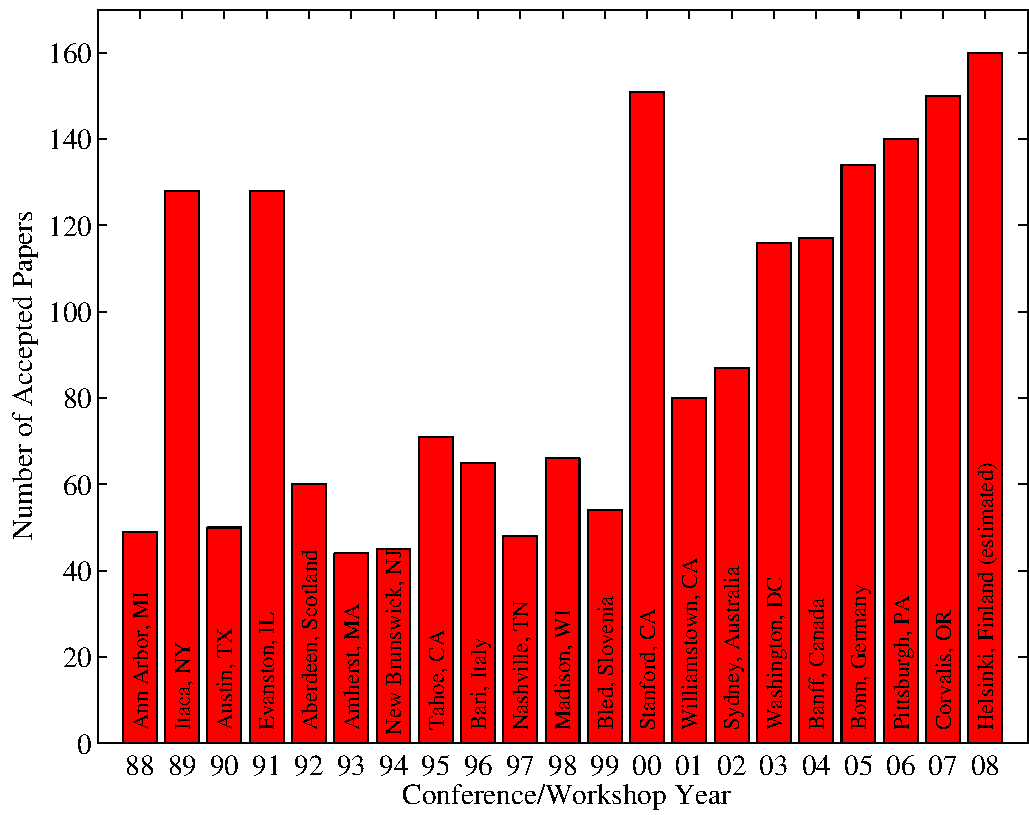
\includegraphics[width=\columnwidth]{icml_numpapers}}
%\caption{Historical locations and number of accepted papers for International
%Machine Learning Conferences (ICML 1993 -- ICML 2008) and International
%Workshops on Machine Learning (ML 1988 -- ML 1992). At the time this figure was
%produced, the number of accepted papers for ICML 2008 was unknown and instead
%estimated.}
%\label{icml-historical}
%\end{center}
%\vskip -0.2in
%\end{figure}

%\subsection{Figures}

%You may want to include figures in the paper to illustrate
%your approach and results. Such artwork should be centered,
%legible, and separated from the text. Lines should be dark and at
%least 0.5~points thick for purposes of reproduction, and text should
%not appear on a gray background.

%Label all distinct components of each figure. If the figure takes the
%form of a graph, then give a name for each axis and include a legend
%that briefly describes each curve. Do not include a title inside the
%figure; instead, the caption should serve this function.

%Number figures sequentially, placing the figure number and caption
%\emph{after} the graphics, with at least 0.1~inches of space before
%the caption and 0.1~inches after it, as in
%Figure~\ref{icml-historical}. The figure caption should be set in
%9~point type and centered unless it runs two or more lines, in which
%case it should be flush left. You may float figures to the top or
%bottom of a column, and you may set wide figures across both columns
%(use the environment \texttt{figure*} in \LaTeX). Always place
%two-column figures at the top or bottom of the page.

%\subsection{Algorithms}

%If you are using \LaTeX, please use the ``algorithm'' and ``algorithmic''
%environments to format pseudocode. These require
%the corresponding stylefiles, algorithm.sty and
%algorithmic.sty, which are supplied with this package.
%Algorithm~\ref{alg:example} shows an example.

%\begin{algorithm}[tb]
   %\caption{Bubble Sort}
   %\label{alg:example}
%\begin{algorithmic}
   %\STATE {\bfseries Input:} data $x_i$, size $m$
   %\REPEAT
   %\STATE Initialize $noChange = true$.
   %\FOR{$i=1$ {\bfseries to} $m-1$}
   %\IF{$x_i > x_{i+1}$}
   %\STATE Swap $x_i$ and $x_{i+1}$
   %\STATE $noChange = false$
   %\ENDIF
   %\ENDFOR
   %\UNTIL{$noChange$ is $true$}
%\end{algorithmic}
%\end{algorithm}

%\subsection{Tables}

%You may also want to include tables that summarize material. Like
%figures, these should be centered, legible, and numbered consecutively.
%However, place the title \emph{above} the table with at least
%0.1~inches of space before the title and the same after it, as in
%Table~\ref{sample-table}. The table title should be set in 9~point
%type and centered unless it runs two or more lines, in which case it
%should be flush left.

%% Note use of \abovespace and \belowspace to get reasonable spacing
%% above and below tabular lines.

%\begin{table}[t]
%\caption{Classification accuracies for naive Bayes and flexible
%Bayes on various data sets.}
%\label{sample-table}
%\vskip 0.15in
%\begin{center}
%\begin{small}
%\begin{sc}
%\begin{tabular}{lcccr}
%\toprule
%Data set & Naive & Flexible & Better? \\
%\midrule
%Breast    & 95.9$\pm$ 0.2& 96.7$\pm$ 0.2& $\surd$ \\
%Cleveland & 83.3$\pm$ 0.6& 80.0$\pm$ 0.6& $\times$\\
%Glass2    & 61.9$\pm$ 1.4& 83.8$\pm$ 0.7& $\surd$ \\
%Credit    & 74.8$\pm$ 0.5& 78.3$\pm$ 0.6&         \\
%Horse     & 73.3$\pm$ 0.9& 69.7$\pm$ 1.0& $\times$\\
%Meta      & 67.1$\pm$ 0.6& 76.5$\pm$ 0.5& $\surd$ \\
%Pima      & 75.1$\pm$ 0.6& 73.9$\pm$ 0.5&         \\
%Vehicle   & 44.9$\pm$ 0.6& 61.5$\pm$ 0.4& $\surd$ \\
%\bottomrule
%\end{tabular}
%\end{sc}
%\end{small}
%\end{center}
%\vskip -0.1in
%\end{table}

%Tables contain textual material, whereas figures contain graphical material.
%Specify the contents of each row and column in the table's topmost
%row. Again, you may float tables to a column's top or bottom, and set
%wide tables across both columns. Place two-column tables at the
%top or bottom of the page.

%\subsection{Citations and References}

%Please use APA reference format regardless of your formatter
%or word processor. If you rely on the \LaTeX\/ bibliographic
%facility, use \texttt{natbib.sty} and \texttt{icml2019.bst}
%included in the style-file package to obtain this format.

%Citations within the text should include the authors' last names and
%year. If the authors' names are included in the sentence, place only
%the year in parentheses, for example when referencing Arthur Samuel's
%pioneering work \yrcite{Samuel59}. Otherwise place the entire
%reference in parentheses with the authors and year separated by a
%comma \cite{Samuel59}. List multiple references separated by
%semicolons \cite{kearns89,Samuel59,mitchell80}. Use the `et~al.'
%construct only for citations with three or more authors or after
%listing all authors to a publication in an earlier reference \cite{MachineLearningI}.

%Authors should cite their own work in the third person
%in the initial version of their paper submitted for blind review.
%Please refer to Section~\ref{author info} for detailed instructions on how to
%cite your own papers.

%Use an unnumbered first-level section heading for the references, and use a
%hanging indent style, with the first line of the reference flush against the
%left margin and subsequent lines indented by 10 points. The references at the
%end of this document give examples for journal articles \cite{Samuel59},
%conference publications \cite{langley00}, book chapters \cite{Newell81}, books
%\cite{DudaHart2nd}, edited volumes \cite{MachineLearningI}, technical reports
%\cite{mitchell80}, and dissertations \cite{kearns89}.

%Alphabetize references by the surnames of the first authors, with
%single author entries preceding multiple author entries. Order
%references for the same authors by year of publication, with the
%earliest first. Make sure that each reference includes all relevant
%information (e.g., page numbers).

%Please put some effort into making references complete, presentable, and
%consistent. If using bibtex, please protect capital letters of names and
%abbreviations in titles, for example, use \{B\}ayesian or \{L\}ipschitz
%in your .bib file.

%\subsection{Software and Data}

%We strongly encourage the publication of software and data with the
%camera-ready version of the paper whenever appropriate. This can be
%done by including a URL in the camera-ready copy. However, do not
%include URLs that reveal your institution or identity in your
%submission for review. Instead, provide an anonymous URL or upload
%the material as ``Supplementary Material'' into the CMT reviewing
%system. Note that reviewers are not required to look at this material
%when writing their review.

%% Acknowledgements should only appear in the accepted version.
%\section*{Acknowledgements}

%\textbf{Do not} include acknowledgements in the initial version of
%the paper submitted for blind review.

%If a paper is accepted, the final camera-ready version can (and
%probably should) include acknowledgements. In this case, please
%place such acknowledgements in an unnumbered section at the
%end of the paper. Typically, this will include thanks to reviewers
%who gave useful comments, to colleagues who contributed to the ideas,
%and to funding agencies and corporate sponsors that provided financial
%support.


%% In the unusual situation where you want a paper to appear in the
%% references without citing it in the main text, use \nocite
%\nocite{langley00}

\bibliography{main}
\bibliographystyle{icml2019}


%%%%%%%%%%%%%%%%%%%%%%%%%%%%%%%%%%%%%%%%%%%%%%%%%%%%%%%%%%%%%%%%%%%%%%%%%%%%%%%%
%%%%%%%%%%%%%%%%%%%%%%%%%%%%%%%%%%%%%%%%%%%%%%%%%%%%%%%%%%%%%%%%%%%%%%%%%%%%%%%%
%% DELETE THIS PART. DO NOT PLACE CONTENT AFTER THE REFERENCES!
%%%%%%%%%%%%%%%%%%%%%%%%%%%%%%%%%%%%%%%%%%%%%%%%%%%%%%%%%%%%%%%%%%%%%%%%%%%%%%%%
%%%%%%%%%%%%%%%%%%%%%%%%%%%%%%%%%%%%%%%%%%%%%%%%%%%%%%%%%%%%%%%%%%%%%%%%%%%%%%%%
%\appendix
%\section{Do \emph{not} have an appendix here}

%\textbf{\emph{Do not put content after the references.}}
%%
%Put anything that you might normally include after the references in a separate
%supplementary file.

%We recommend that you build supplementary material in a separate document.
%If you must create one PDF and cut it up, please be careful to use a tool that
%doesn't alter the margins, and that doesn't aggressively rewrite the PDF file.
%pdftk usually works fine. 

%\textbf{Please do not use Apple's preview to cut off supplementary material.} In
%previous years it has altered margins, and created headaches at the camera-ready
%stage. 
%%%%%%%%%%%%%%%%%%%%%%%%%%%%%%%%%%%%%%%%%%%%%%%%%%%%%%%%%%%%%%%%%%%%%%%%%%%%%%%%
%%%%%%%%%%%%%%%%%%%%%%%%%%%%%%%%%%%%%%%%%%%%%%%%%%%%%%%%%%%%%%%%%%%%%%%%%%%%%%%%


\end{document}
